\documentclass[12pt, twoside, openright]{report} %fuente a 12pt, formato doble pagina y chapter a la derecha
\raggedbottom % No ajustar el contenido con un salto de pagina

% MÁRGENES: 2,5 cm sup. e inf.; 3 cm izdo. y dcho.
\usepackage[
a4paper,
vmargin=2.5cm,
hmargin=3cm
]{geometry}

% INTERLINEADO: Estrecho (6 ptos./interlineado 1,15) o Moderado (6 ptos./interlineado 1,5)
\renewcommand{\baselinestretch}{1.15}
\parskip=6pt

% DEFINICIÓN DE COLORES para portada y listados de código
\usepackage[table]{xcolor}
\definecolor{azulUC3M}{RGB}{0,0,102}
\definecolor{gray97}{gray}{.97}
\definecolor{gray75}{gray}{.75}
\definecolor{gray45}{gray}{.45}

% Soporte para GENERAR PDF/A
\usepackage[a-1b]{pdfx}

% ENLACES
\usepackage{hyperref}
\hypersetup{colorlinks=true,
	linkcolor=black, % enlaces a partes del documento (p.e. índice) en color negro
	urlcolor=blue} % enlaces a recursos fuera del documento en azul

% Añadir pdfs como partes del documento
\usepackage{pdfpages}

% Quitar la indentación de principio de los parrafos
\setlength{\parindent}{0em}

% EXPRESIONES MATEMATICAS
\usepackage{amsmath,amssymb,amsfonts,amsthm}

\usepackage{txfonts} 
\usepackage[T1]{fontenc}
\usepackage[utf8]{inputenc}

% Insertar graficas y fotos
\usepackage{tikz}
\usepackage{pgfplots}

\usepackage[spanish, es-tabla]{babel} 
\usepackage[babel, spanish=spanish]{csquotes}
\AtBeginEnvironment{quote}{\small}

% diseño de PIE DE PÁGINA
\usepackage{fancyhdr}
\pagestyle{fancy}
\fancyhf{}
\renewcommand{\headrulewidth}{0pt}
\fancyfoot[LE,RO]{\thepage}
\fancypagestyle{plain}{\pagestyle{fancy}}

% DISEÑO DE LOS TÍTULOS de las partes del trabajo (capítulos y epígrafes o subcapítulos)
\usepackage{titlesec}
\usepackage{titletoc}
\titleformat{\chapter}[block]
{\large\bfseries\filcenter}
{\thechapter.}
{5pt}
{\MakeUppercase}
{}
\titlespacing{\chapter}{0pt}{0pt}{*3}
\titlecontents{chapter}
[0pt]                                               
{}
{\contentsmargin{0pt}\thecontentslabel.\enspace\uppercase}
{\contentsmargin{0pt}\uppercase}                        
{\titlerule*[.7pc]{.}\contentspage}                 

\titleformat{\section}
{\bfseries}
{\thesection.}
{5pt}
{}
\titlecontents{section}
[5pt]                                               
{}
{\contentsmargin{0pt}\thecontentslabel.\enspace}
{\contentsmargin{0pt}}
{\titlerule*[.7pc]{.}\contentspage}

\titleformat{\subsection}
{\normalsize\bfseries}
{\thesubsection.}
{5pt}
{}
\titlecontents{subsection}
[10pt]                                               
{}
{\contentsmargin{0pt}                          
	\thecontentslabel.\enspace}
{\contentsmargin{0pt}}                        
{\titlerule*[.7pc]{.}\contentspage}  


% DISEÑO DE TABLAS.
\usepackage{multirow} % permite combinar celdas 
\usepackage{caption} % para personalizar el título de tablas y figuras
\usepackage{floatrow} % utilizamos este paquete y sus macros \ttabbox y \ffigbox para alinear los nombres de tablas y figuras de acuerdo con el estilo definido. Para su uso ver archivo de ejemplo 
\usepackage{array} % con este paquete podemos definir en la siguiente línea un nuevo tipo de columna para tablas: ancho personalizado y contenido centrado
\newcolumntype{P}[1]{>{\centering\arraybackslash}p{#1}}
\DeclareCaptionFormat{upper}{#1#2\uppercase{#3}\par}

% Diseño de tabla para ingeniería
\captionsetup[table]{
	format=hang,
	name=Tabla,
	justification=centering,
	labelsep=colon,
	width=.75\linewidth,
	labelfont=small,
	font=small,
}

% DISEÑO DE FIGURAS.
\usepackage{graphicx}
\graphicspath{{img/}} %ruta a la carpeta de imágenes

% Diseño de figuras para ingeniería
\captionsetup[figure]{
	format=hang,
	name=Fig.,
	singlelinecheck=off,
	labelsep=colon,
	labelfont=small,
	font=small		
}

% NOTAS A PIE DE PÁGINA
\usepackage{chngcntr} %para numeración continua de las notas al pie
\counterwithout{footnote}{chapter}

% LISTADOS DE CÓDIGO
% soporte y estilo para listados de código. Más información en https://es.wikibooks.org/wiki/Manual_de_LaTeX/Listados_de_código/Listados_con_listings
\usepackage{listings}

% definimos un estilo de listings
\lstdefinestyle{estilo}{ frame=Ltb,
	framerule=0pt,
	aboveskip=0.5cm,
	framextopmargin=3pt,
	framexbottommargin=3pt,
	framexleftmargin=0.4cm,
	framesep=0pt,
	rulesep=.4pt,
	backgroundcolor=\color{gray97},
	rulesepcolor=\color{black},
	%
	basicstyle=\ttfamily\footnotesize,
	keywordstyle=\bfseries,
	stringstyle=\ttfamily,
	showstringspaces = false,
	commentstyle=\color{gray45},     
	%
	numbers=left,
	numbersep=15pt,
	numberstyle=\tiny,
	numberfirstline = false,
	breaklines=true,
	xleftmargin=\parindent
}

\captionsetup[lstlisting]{font=small, labelsep=period}
% fijamos el estilo a utilizar 
\lstset{style=estilo}
\renewcommand{\lstlistingname}{\uppercase{Código}}

\pgfplotsset{compat=1.17} 
%-------------
%	DOCUMENTO
%-------------

\begin{document}
\pagenumbering{roman} % Se utilizan cifras romanas en la numeración de las páginas previas al cuerpo del trabajo
	
%----------
%	PORTADA
%----------	
\begin{titlepage}
	\begin{sffamily}
	\color{azulUC3M}
	\begin{center}
		\begin{figure}[H] %incluimos el logotipo de la Universidad
			\makebox[\textwidth][c]{
\includegraphics[width=16cm]{Portada_Logo.png}}
		\end{figure}
		\vspace{2.5cm}
		\begin{Large}
			Grado en Ingeniería Informática\\			
			2020-2021\\
			\vspace{2cm}		
			\textsl{Apuntes}\\
			\bigskip
		\end{Large}
		 	{\Huge Interfaces de Usuario}\\
		 	\vspace*{0.5cm}
	 		\rule{10.5cm}{0.1mm}\\
			\vspace*{0.9cm}
			{\LARGE Jorge Rodríguez Fraile\footnote{\href{mailto:100405951@alumnos.uc3m.es}{Universidad: 100405951@alumnos.uc3m.es}  |  \href{mailto:jrf1616@gmail.com}{Personal: jrf1616@gmail.com}}}\\ 
			\vspace*{1cm}
	\end{center}
	\vfill
	\color{black}
		
\includegraphics[width=4.2cm]{img/creativecommons.png}\\
		Esta obra se encuentra sujeta a la licencia Creative Commons\\ \textbf{Reconocimiento - No Comercial - Sin Obra Derivada}
	\end{sffamily}
\end{titlepage}

%----------
%	ÍNDICES
%----------	

%--
% Índice general
%-
\tableofcontents
\thispagestyle{fancy}

%--
% Índice de figuras. Si no se incluyen, comenta las líneas siguientes
%-
\listoffigures
\thispagestyle{fancy}

%----------
%	TRABAJO
%----------	

\pagenumbering{arabic} % numeración con múmeros arábigos para el resto de la publicación	


%----------
%	COMENZAR A ESCRIBIR AQUI
%----------	

\chapter{Información}
\section{Profesores}
\begin{quote}
Magistral: Ana Tajadura Jiménez

Prácticas: Teresa Onorati tonorati@uc3m.es Tutorías: Martes 12:30-14:00
\end{quote}

\section{Recursos}

Tutoriales de HTML en \href{https://www.w3schools.com/}{W3Schools Online Web Tutorials}

Página para poder trabajar online en HTML en: \href{https://repl.it/}{The collaborative browser based IDE}

\begin{itemize}

\item
  El cliente pide información al servido, este se la entrega y la
  muestra al cliente. Se realiza mediante el protocolo HTTP.
\item
  Protocolo HTTP: En la arquitectura cliente servidor, el cliente envía
  datos al servidor a través del protocolo HTTP. El servidor responde
  con la información solicitada codificada en HTML. El cliente
  interpreta el código HTML, ya que hay por ejemplo diferentes horas
  según el país.
\item
  El cliente se conecta mediante una URL - Uniform Resource Locator,
  secuencia de caracteres que sigue un formato estándar y que se usa
  para localizar recursos en los servidores.
\end{itemize}

\part{Teoría}


\chapter{TEMA 1 - Interacción Persona-Ordenador}
Estamos desde el punto de vista del usuario, para ver como de
    accesible y fáciles de usar son los productos interactivos.

    \begin{itemize}
    
    \item
      Primero se llamó Man-Machine Interface, después Human-Computer
      Interaction - HCI o IPO.
    \end{itemize}

	Los productos interactivos: Aquellos que al recibir datos del
    usuario realizan acciones o devuelven un resultado. Pueden tener
    diferente tamaño, uso y características.

    \begin{itemize}
    \item
      Un lenguaje de entrada para el usuario, de salida para el sistema
      y un protocolo de interacción.
    \end{itemize}

	Los productos están diseñados para desempeñar una tarea, pero no
    siempre se tiene en cuentas las personas reales que los utilizan,
    hay que tener en cuenta quien y como lo van a utilizar.

	Lo primero es pensar en el usuario, saber a quién va dirigido y
    escuchar sus necesidades.

    \begin{itemize}
    
    \item
      Factores:

      \begin{itemize}
      
      \item
        Visibilidad.
      \item
        Causalidad.
      \item
        Restricciones visibles.
      \item
        Coincidencia (``Mapping''): Debe reflejar la relación natural
        entre las cosas (Que se pueda asociar observando)
      \item
        Efectos de transferencia.
      \item
        Estereotipos de los usuarios.
      \item
        Modelos conceptuales.
      \item
        Diferencias individuales, culturales.
      \end{itemize}
    \item
      Los controles necesitan ser visibles (visibilidad) con una buena
      representación de sus efectos (causalidad), y su diseño debería
      sugerir su funcionalidad (mapping).
    \item
      La gente tiene modelos mentales de cómo funcionan las cosas por
      asociación con otras y pueden simular mentalmente la operación,
      pero pueden ser erróneos y hay que buscar un equilibrio entre
      utilidad y diseño.

      \begin{itemize}
      
      \item
        Ejem: Buen IPO Volante, deja simple un sistema complejo. Mal IPO
        Control video, no se asocia lo que hace con los símbolos.
      \end{itemize}
    \end{itemize}

	La primera IPO fue con el ratón, que permitía interactuar con el
    sistema mediante un dispositivo externo con una interfaz.

	El objetivo de la IPO es desarrollar o mejorar:

    \begin{itemize}
    
    \item
      Seguridad -- en el trabajo.
    \item
      Utilidad -- qué puede hacer el sistema.
    \item
      Efectividad -- Lograr su función.
    \item
      Eficiencia -- Emplear menos recursos.
    \item
      Usabilidad o la capacidad de ser usados -- fácil de usar, fácil
      aprendizaje y libre de errores.

      \begin{itemize}
      
      \item
        Para obtener una buena usabilidad, es necesario encontrar los
        factores que determinen como se usan, desarrollar las
        herramientas y técnicas que ayuden a los diseñadores a crear
        sistemas eficientes, efectivos y seguros para el usuario.

		\begin{figure}[H]
			\ffigbox[\FBwidth]
			{\caption{Objetivos de la IPO - HCI}}
			{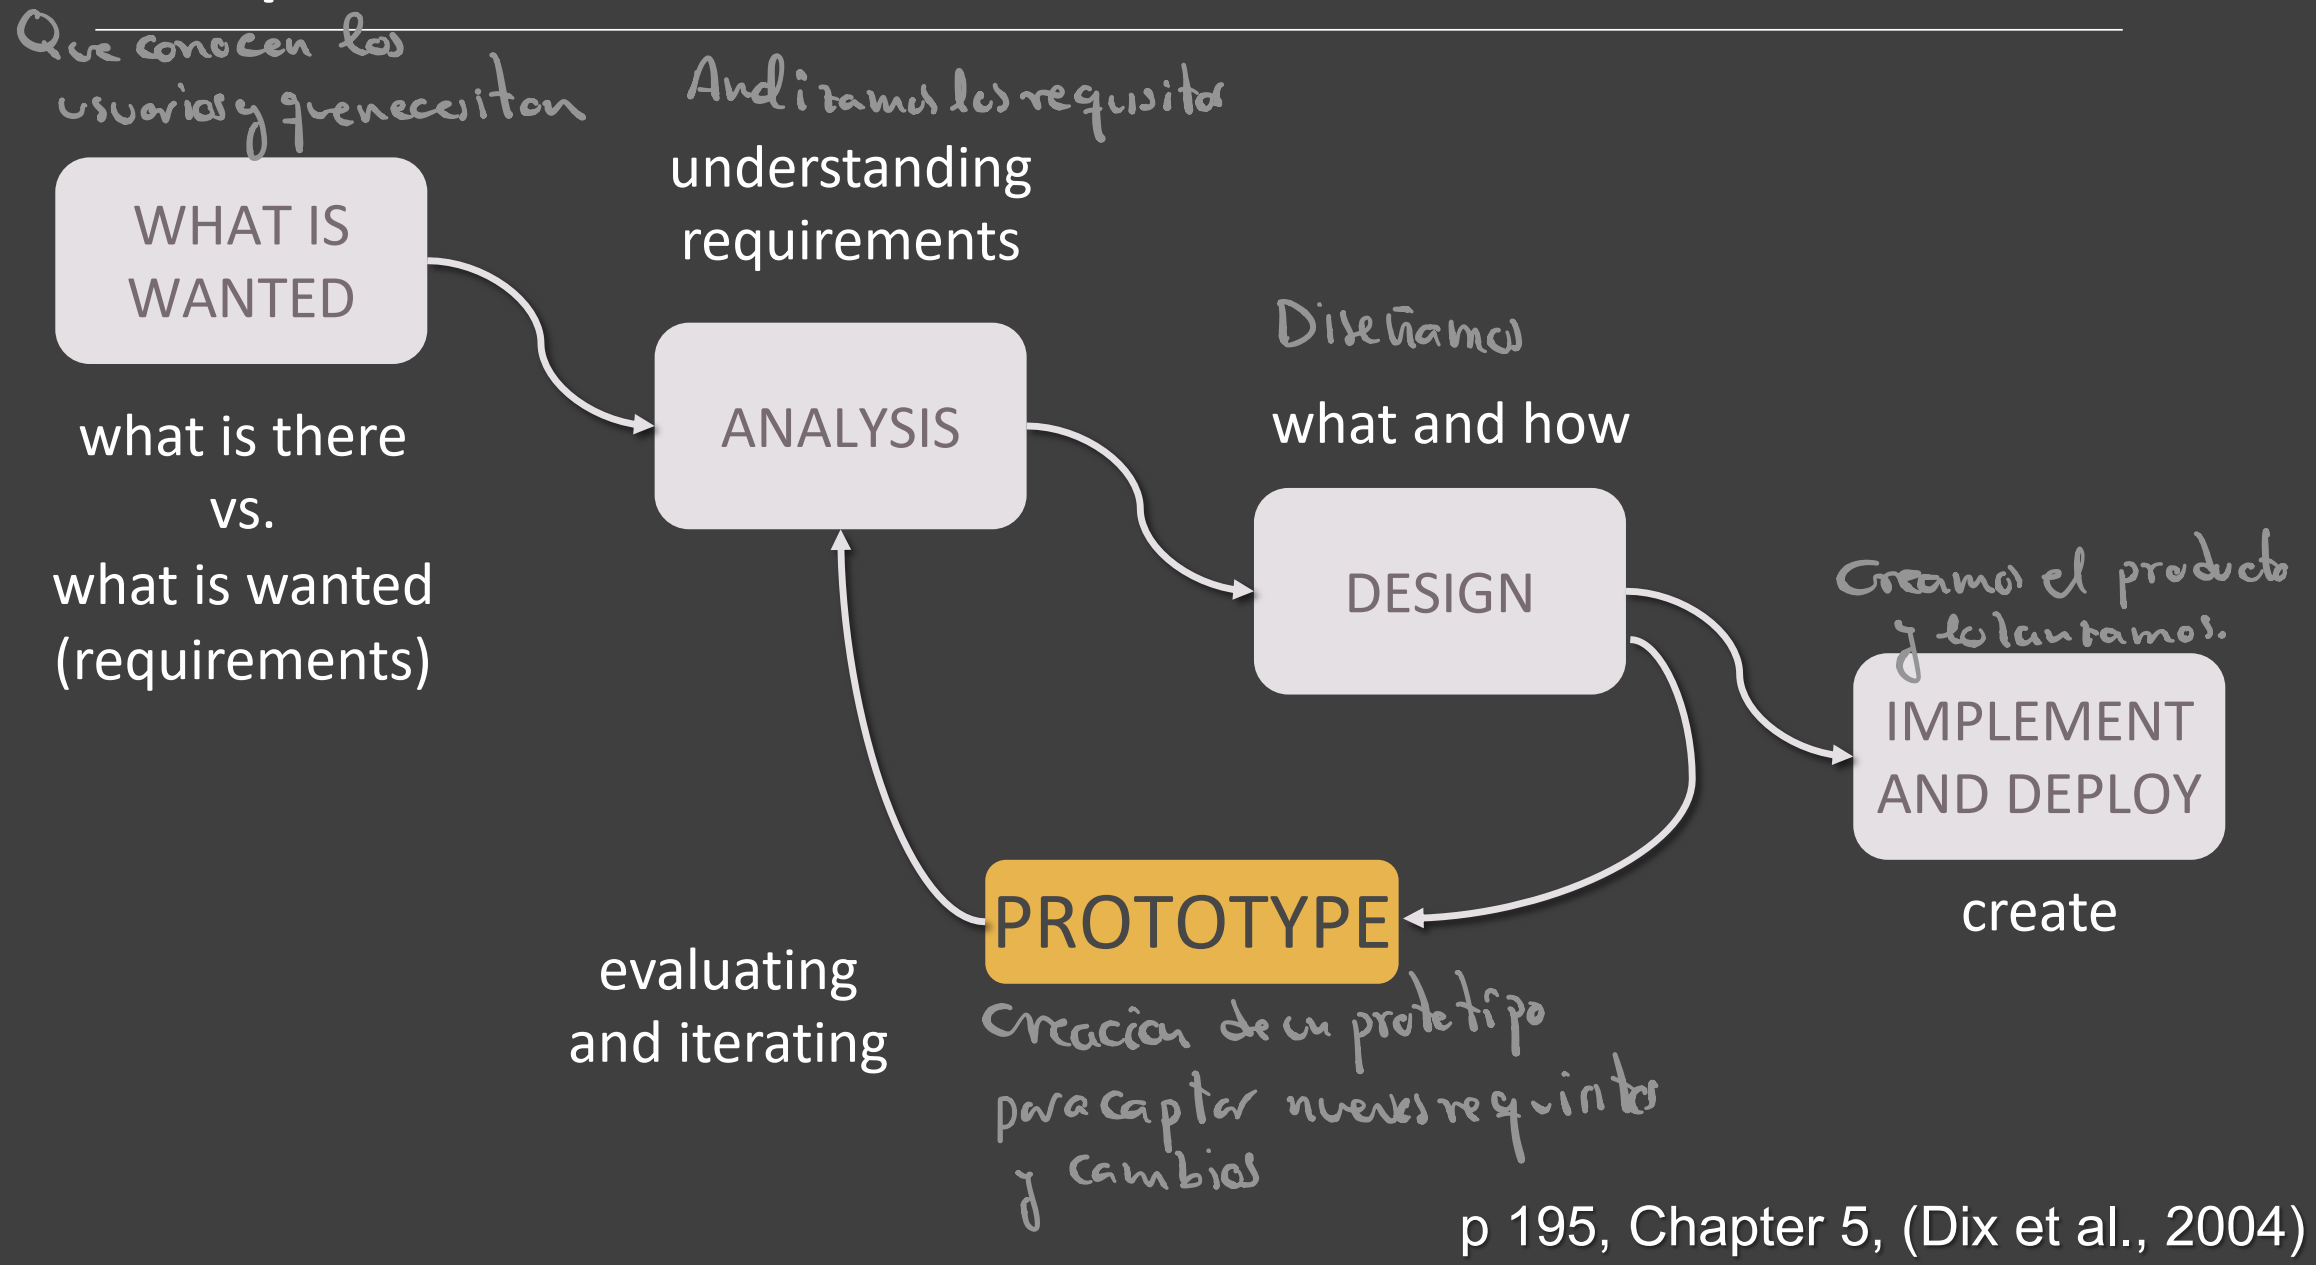
\includegraphics[scale=.17]{Untitled 3.png}}
		\end{figure}
       
      \end{itemize}
    \end{itemize}
\pagebreak
	Factores relacionados con HCI
	\begin{table}[h]
		\begin{tabular}{|c|c|c|c|}
		\hline
		\multicolumn{2}{|c|}{Organization}   & \multicolumn{2}{c|}{Environmental}   \\ \hline
		Health / Security        & \multicolumn{2}{c|}{User} & Ergonomics           \\ \hline
		\multicolumn{4}{|c|}{User interface}                                        \\ \hline
		\multicolumn{4}{|c|}{Task}                                                  \\ \hline
		\multicolumn{4}{|c|}{Restrictions}                                          \\ \hline
		\multicolumn{4}{|c|}{System}                                                \\ \hline
		\multicolumn{4}{|c|}{Productivity}                                          \\ \hline
		\end{tabular}
		\end{table}
   

    Es multidisciplinar, implica diseño, evaluación e implementación
    sistemas interactivos y el estudio de los grandes fenómenos
    alrededor del dicho sistema.

    \begin{itemize}
    
    \item
      Sociología - Entender como la estructura social y la organización
      de las personas afectan a la manera de las personas de realizar
      las tareas.
    \item
      Psicología - El comportamiento humano y sus procesos mentales.
    \item
      Ciencias de la información - Lenguaje e internacionalización.
    \item
      Computer Science - Entender la tecnología y técnicas de diseño,
      desarrollo y administración de sistemas de ordenadores
    \item
      Ergonomía o factores humanos - Adaptarse a las capacidades de los
      humanos, vista, peso, altura, etc.
    \end{itemize}

	Interacción: Es el proceso de comunicación que se establece entre el
    usuario y el sistema. Es un diálogo para completar una tarea.

    \begin{itemize}
    
    \item
      El sistema realiza, simplifica o da soporte a alguna tarea.
    \item
      La interfaz funciona como intermediario entre ambos, mediante ella
      se produce la comunicación y debe diseñarse para que la
      interacción tenga éxito.
    \end{itemize}

	Modelo: Es una representación abstracta de una realidad compleja que
    se utiliza para facilitar su compresión y el estudio de su
    comportamiento. Simplifican los factores a tener en cuenta. Los hay
    de muchos tipos.

	\pagebreak
\section{Modelos de interacción}

 

    Algunos ayudan a comprender el proceso de interacción, otros a
    identificar los problemas que se pueden producir, pero ambos
    simplifican la tarea de pensar en todos los posibles factores que
    pueden afectar a la interacción, siguiendo solo unas pautas.

	Términos:

    \begin{itemize}
    
    \item
      Dominio: Área de habilidad y conocimiento en alguna actividad del
      mundo real. Área de personas que engloba.
    \item
      Meta: Qué se quiere conseguir.
    \item
      Tarea: Cómo quieres conseguir tu meta, por medio de qué o haciendo
      qué.
    \item
      Acciones: Tarea que no implica la resolución de problemas.
    \item
      Plan: Conjunto de tareas para conseguir una meta.
    \end{itemize}

\section{Modelo de Norman}
\vspace{-0.5cm}
    Se basa en: Ejecución y Evaluación.

    \begin{itemize}
    
    \item
      El usuario formula un plan de acciones que ejecuta utilizado la
      interfaz del sistema.
    \item
      Cuando el plan, o parte del plan, se ha ejecutado, el usuario
      observa la interfaz para evaluar el resultado y comprobar si hacen
      falta más acciones.
    \end{itemize}

	Hay dos lenguajes:
	\vspace{-0.5cm}

    \begin{itemize}
    
    \item
      Lenguaje del sistema: El del núcleo, representa el estado del
      sistema.
    \item
      Lenguaje del usuario: El de la tarea, representa el estado del
      usuario.
    \end{itemize}

	Ciclo:
	\vspace{-0.5cm}

    \begin{enumerate}
    \def\labelenumi{\arabic{enumi}.}
    
    \item
      Establecer meta.
    \item
      Formular intención.
    \item
      Especificar las acciones que nos moverán a través de la interfaz.
    \item
      Ejecutar las acciones.
    \item
      Percibir el estado del mundo.
    \item
      Interpretar el estado del mundo.
    \item
      Evaluar el estado del mundo respecto a la meta.
    \end{enumerate}

	Problemas para el usuario:

    \begin{itemize}
    
    \item
      Abismo de ejecución (execution gulf): Diferencia entre las
      acciones que el usuario quiere realizar para alcanzar su objetivo
      y las que el sistema permite.
    \item
      Abismo de evaluación (evaluation gulf): Diferencia entre la
      presentación física del estado del sistema y lo que esperaba el
      usuario.
    \item
      Distancia semántica: La relación entre el significado de los
      elementos en la interfaz y el objetivo que el usuario quiere. La
      diferencia entre lo que hace ese elemento y lo esperábamos por su
      representación
    \item
      Distancia articulada: El número de acciones de más que requiere
      una acción de las pensadas con respecto al significado de los
      elementos de la interfaz.
    \end{itemize}

\section{Modelo de Abowd \& Beale}

  \begin{itemize}
  
  \item
    Respecto al modelo de Norman se influye la IU de forma explícita,
    que realiza la traducción entre lenguaje de usuario y lenguaje del
    sistema y viceversa.
	\begin{figure}[H]
		\ffigbox[\FBwidth]
		{\caption{Abowd \& Beale}}
		{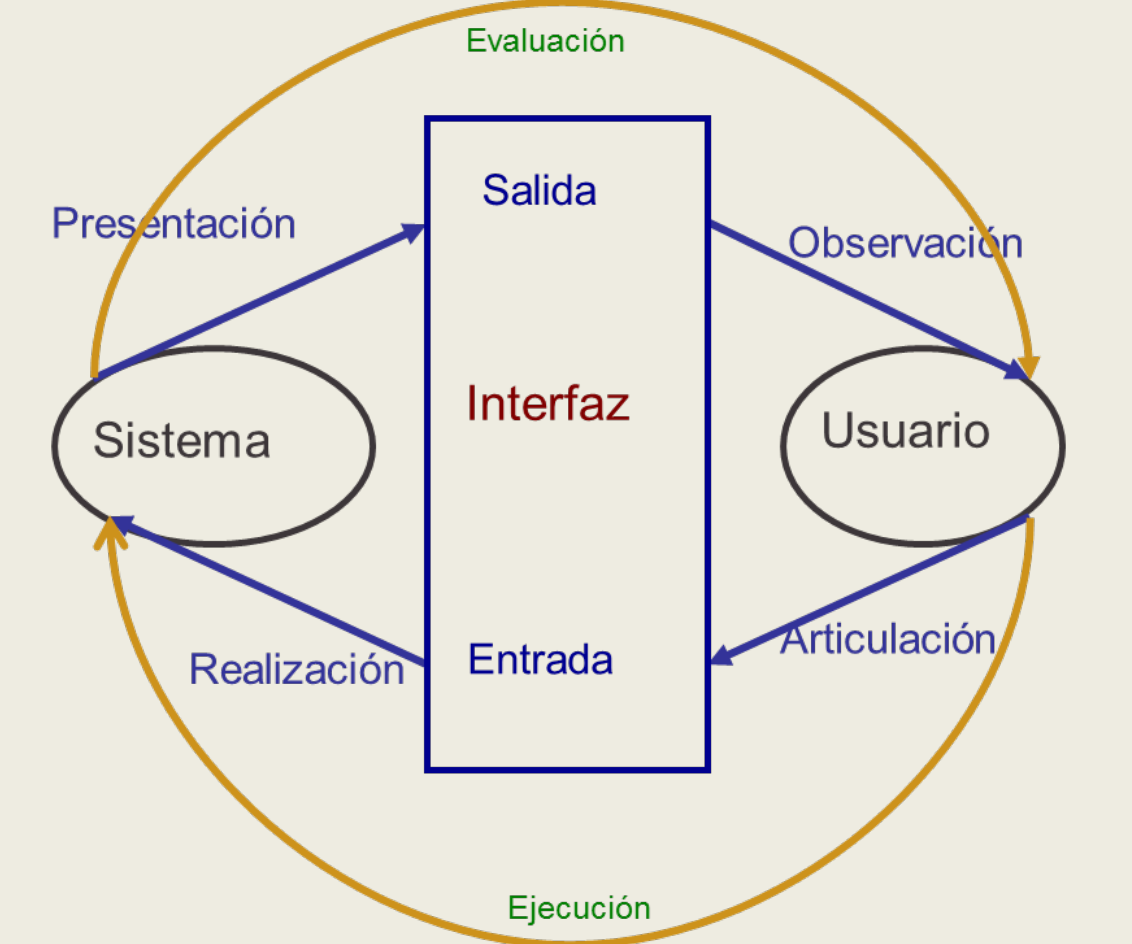
\includegraphics[scale=.3]{Untitled 2.png}}
	\end{figure}
  \end{itemize}

\chapter{TEMA 2 - Interfaces de Usuario}

\section{Interfaz de usuario}

    Es el canal a través del cual se produce la comunicación entre el
    usuario y el ordenador, física (ergonómica) en dispositivos y Lógica
    (usable y fácil) en dispositivos y sistemas. La interacción es un
    diálogo para completar una tarea.

	Debe ser diseñada para ser eficiente y satisfactoria. El diálogo lo
    más fluido posible.

	Es importante para transformar la complejidad tecnológica en un
    producto útil, utilizable y atractivo para sus usuarios.

	Tipos:

    \begin{itemize}
    
    \item
      Textual.
    \item
      Gráfica
    \item
      Multimedia
    \item
      Multimodal
    \item
      Conversacional
    \end{itemize}

\subsection{Tipos de interfaces interactivas:}

\subsubsection{Comandos}
Cada comando se ejecuta en un terminal y el sistema
      responde con el resultado correspondiente.

      \begin{itemize}
      
      \item
        Eficiente, precisa y veloz, a pesar de ser difícil de aprender.
      \item
        Utilizada como alternativa para personas con discapacidad
        visual.
      \end{itemize}
\pagebreak
	 \subsubsection{WIMP y GUI -- Graphic User Interface} 

        Ventanas: Se puede minimizar, maximizar, cambiar el tamaño y
        estilo.

        \begin{itemize}
        
        \item
          Se inventaron para superar las limitaciones físicas de la
          pantalla de un ordenador para visualizar más información y
          ejecutar más tareas.
        \item
          Si se abren demasiadas ventanas podrían resultar difícil de
          gestionar, para ello se pueden reducir a un icono en la barra
          de tareas, listar todas o moverse fácilmente.
        \item
          Tipos:

          \begin{itemize}
          
          \item
            Tiled Windows: Ventanas en forma de baldosas, que se pueden
            coger y arrastrar.
          \item
            Overlapping Windows: Ventanas sobrepuestas, hace uso
            eficiente de todo el espacio de la pantalla, pero difícil de
            manejar.
          \item
            Cascading Windows: Ventanas en cascada, hace uso eficiente
            de todo el espacio de la pantalla y fácilmente organizables.
          \end{itemize}
        \item
          Posibles interfaces:

          \begin{itemize}
          
          \item
            Multiple Document Interface -- MDI:

            \begin{itemize}
            
            \item
              Centrada en la aplicación.
            \item
              Una aplicación lanza una ventana principal que funciona
              como espacio de trabajo para todos los documentos.
            \item
              Las ventanas hijo pueden minimizarse dentro de los padres.
            \item
              Ventajas:

                Recursos del sistema se conservan.

				No abarrotamiento visual.

				Ver múltiples documentos a la vez.

				\item
              Desventajas:

                Los menús cambian según el documento.

				Todos los documentos dentro del área de trabajo.

				Las ventanas hijo están dentro del padre y puede ser
                complejo visualmente.

			\end{itemize}
          \item
            Single Document Interface -- SDI:

            \begin{itemize}
            
            \item
              Centrada en el documento. Una ventana para cada documento.
            \item
              Ventajas:
			  
                Todos los menús y barras de herramientas reflejan la
                visión del usuario.

				Menos complejo visualmente.

				\item
              Desventajas:

                No se pueden agrupar ventanas, las barra de tareas puede
                aparecer llena.

				La transición entre ventanas puede ser compleja.

			\end{itemize}
          \item
            Tabbed Document Interface -- TDI:

            \begin{itemize}
            
            \item
              Variante de MDI.
            \item
              Incorpora el uso de pestañas para cambiar entre
              documentos.
            \item
              Algunas fijas el tamaño a máximo y otras permiten cambiar
              el tamaño y minimizar las ventanas de documento y se
              convierten en MDI.
            \end{itemize}
          \item
            Cajas de diálogo:

            \begin{itemize}
            
            \item
              Espacio en el que llevar a cabo funcionalidades
              relacionadas pero secundarias, como:

                Gestionar las propiedades de un objeto

				Ejecutar funciones o procesos

				Confirmar acciones

				Alertar errores.

				\item
              Pueden ser:
			  
                Modales: El usuario no puede hacer otra cosa hasta que
                haya terminado las acciones por la que se abrió.

				No modales: El usuario puede acceder a otras
                funcionalidades del programa mientras el diálogo está
                abierto.

				\item
              Se pueden encadenar cajas de diálogo para proporcionar
              acceso a funcionalidades avanzadas.
            \end{itemize}
          \item
            Otros elementos:

            \begin{itemize}
            
            \item
              Paneles:
			  
                Agrupación visual de funcionalidades relacionadas.

				Forma eficiente de acceder a las funcionalidades sin
                usar menús.

				\item
              Marcos:
			  
                Pueden minimizarse y cambiarse de tamaño.

				Suelen usarse para separar áreas de navegación.

				\item
              Pestañas:
                Permiten incrementar el tamaño del diálogo apilando
                niveles y facilitan que se acceda a más elementos.

			\end{itemize}
          \end{itemize}
        \end{itemize}
\pagebreak
		Iconos: Representan aplicaciones, objetos, comandos y
        herramientas que se pueden ejecutar al hacer clic.

        \begin{itemize}
        
        \item
          Son más fáciles de aprender y recordar que los comandos. Son
          muy utilizados.
        \item
          Ocupan poco espacio y permiten moverse en la pantalla.
        \item
          Tipos:

          \begin{itemize}
          
          \item
            Similar:
          \item
            Analógica: Se asocia mentalmente.
          \item
            Arbitraria: No hay relación.
          \end{itemize}
        \end{itemize}

		Menús: Lista de opciones que pueden ser exploradas.

        \begin{itemize}
        
        \item
          Tipos:

          \begin{itemize}
          
          \item
            Listas: Ideal pocas opciones que se quieren visualizar al
            mismos tiempo y en una pantalla pequeña.
          \item
            Expansible: Ideal para muchas opciones. Enseñar múltiples
            opciones en una sola pantalla.
          \item
            Contextual: Las opciones ofrecidas dependen del contexto de
            la tarea.
          \end{itemize}

	\item
        Puntero: Un ratón lo controla para entrar en una ventana, un
        menú o unos iconos en pantalla.
      \item
        El nuevo objetivo es diseñar interfaces óptimas para tablets,
        smartphones y smartwatches.
      \end{itemize}

\subsubsection{Multimedia}	  

Combinación de diferentes medias en la misma interfaz ofreciendo
        distintos modos de interactuar.

		Facilita el acceso a diferentes tipos de información.

		Mejora el aprendizaje y al aceptación por parte de los usuarios.

\subsubsection{Realidad Virtual}

      
		
        Es una simulación gráfica generada por ordenador que genera la
        ilusión de participar en un entorno no real.

		Los usuarios pueden interactuar con los objetos y navegar en un
        entorno 3D con un alto sentido de presencia.
\subsubsection{Tableros gráficos}

        Utilizados para visualizar datos complejos.

		Mejoran la capacidad de pensamiento y aprendizaje de los
        usuarios que pueden reconocer patrones o anomalías en los datos.

		Técnicas:

        \begin{itemize}
        
        \item
          Mapas interactivos 3D.
        \item
          Árboles
        \item
          Clústeres
        \end{itemize}

		Hay que tomar decisiones de diseño para ofrecer la información
        de la mejor manera.

\subsubsection{Movil}
        Pensados para utilizarse en movimiento a lo largo del día.

		Hay que tener en cuenta las reducidas dimensiones de las
        pantallas.

		Muchas aplicaciones son para la diversión y no contestar una
        necesidad.

\subsubsection{Voz}

        Se utiliza para acceder algún tipo específico de información.

		También para facilitar la interacción con personas con algún
        tipo de discapacidad.

\subsubsection{Compartida}
        Diseñadas para ser utilizadas por más usuarios y recibir varios
        inputs al mismo tiempo.

		Se suelen utilizar pantallas de grandes dimensiones, deben tener
        en cuenta el tamaño de las pantallas

\subsubsection{Cerebro-ordenador}

      \begin{itemize}
      
      \item
        Permiten establecer una comunicación bidireccional entre las
        ondas cerebrales del usuario y un dispositivo exterior.
      \item
        Se utilizan para juegos o para permitir a las personas
        paralelizadas.
      \item
        Los usuarios deben estar concentrados, ya que detecta cambios en
        las funcione neuronales.
      \end{itemize}

	La interfaz que debemos utilizar depende del tipo de tarea, usuario,
    contexto, coste, características que se quieren garantizar.

	También hay que tener en cuenta que hoy en día los móviles se
    utilizan más que los ordenadores, queremos hacer más cosas al mismo
    tiempo y se usan interfaces basadas en comando vocales.

	Las interfaces compartidas y táctiles son bastante comunes en
    espacios como casas, escuelas, lugares públicos y de trabajo.

	
\section{Usabilidad}

  El primer diseño no es el bueno, hay que implicar al usuario e iterar
  la consulta al usuario y el diseño.

  
    Usabilidad: Es la cualidad de un sistema respecto a la facilidad de
    uso, la facilidad de aprendizaje y la satisfacción del usuario.
    Fácil de usar, fácil de aprender, efectivo, eficiente, útil y
    seguro.

	Es la propiedad que refleja la facilidad de uso de un sistema
    informático.

    \begin{itemize}
    
    \item
      Un buen diseño hace que sea fácil de entender y utilizar.
    \item
      Un diseño pobre hace que sea difícil de utilizar
    \end{itemize}

	Beneficios:

    \begin{itemize}
    
    \item
      Reducción de costes de aprendizaje, de asistencia y ayuda al
      usuario.
    \item
      Mejora la aceptación, la calidad de vida de los usuarios, el
      prestigio y la imagen del sistema.
    \item
      Reducción de los costes de producir y aumento de la productividad.
    \end{itemize}

	Usabilidad vs. User Experience:

    \begin{itemize}
    
    \item
      La experiencia del usuario representa todos los aspectos de la
      interacción del usuario final con la empresa, servicio y
      productos.
    \item
      La usabilidad representa lo fácil de aprender, eficiente de usar,
      agradable de un producto. La experiencia total es más amplia.
    \end{itemize}
\pagebreak
    Es necesario que el sistema hable el mismo lenguaje del usuario:

    \begin{itemize}
    
    \item
      Demasiadas opciones representan una carga adicional de
      información, el usuario tendrá que hacer un esfuerzo extra para
      aprender, entender y buscar.
    \item
      La información, así como las funcionalidades del sistema se deben
      presentar con un lenguaje natural e iconos fáciles de entender.
    \item
      Hay que garantizar una correspondencia entre lo que visualiza el
      sistema y el modelo metal del usuario.
    \item
      Hay que analizar las necesidades del usuario y su entorno.
    \end{itemize}

	El diseño de la interfaz de usuario se basa en el uso de diferentes
    metáforas:

    \begin{itemize}
    
    \item
      Las metáforas podrían tener problemas de internacionalización.
    \item
      Hay que tener en cuenta el bagaje cultural de los usuarios.
    \item
      Las evaluaciones con los usuarios son necesarias para valorar el
      significado de las metáforas definidas.
    \end{itemize}

	Hay que tener en cuenta varios factores relacionados con el ser
    humano para poder diseñar una interfaz usable:

    
\subsection{La percepción visual}
Depende del ángulo de visión, nos permite
      conocer el tamaño y de la profundidad de un objeto.

      \begin{itemize}
      
      \item
        Leyes de la Gestalt: Son un conjunto de principios sobre como
        las personas perciben y organizan los elementos.

        \begin{itemize}
        
        \item
          Ley de cierre: La imaginación tiende a completar las imágenes.
        \item
          Ley de la figura y fondo: El fondo tiende a no ser percibido.
        \item
          Ley de la simplicidad: Los elementos se perciben de la forma
          más simple.
        \end{itemize}
      \item
        Brillo: Cantidad de luminancia perceptible que proporciona un
        objeto.

        \begin{itemize}
        
        \item
          Mayor luminancia más agudeza visual y frecuencia de parpadeo.
        \end{itemize}
      \item
        Contraste: Relación entre el brillo del texto y el del fondo.

        \begin{itemize}
        
        \item
          El contraste negativo se lee mejor, pero produce más
          cansancio.
        \end{itemize}
      \item
        Color: Compuesto por matiz, intensidad y saturación ( cantidad
        de blanco).

        \begin{itemize}
        
        \item
          Se aconseja usar entre 5 y 7 colores, los grises más idóneos.
        \item
          Debe ser accesible en blanco y negro.
        \item
          Utilizar para categorizar, diferenciar o evidenciar.
        \item
          Teoría del color: No existe una receta para hacer buenas
          combinaciones de colores, pero si propiedades.

          \begin{itemize}
          
          \item
            Colores primarios: Amarillo, rojo y azul.
          \item
            Colores complementarios: Aquellos que están opuestos en el
            circulo cromático que generan gran contraste.
          \item
            Colores análogos: Colores a ambos lados de cualquier color.
            Son la base de los esquemas armónicos.
          \item
            Tríada: 3 colores equidistantes. Armónico y con contraste.
          \item
            Split complementario: Un color y los adyacentes a su
            complementario. Mucho contraste.
          \item
            Tetradica: Dos colores y sus complementarios
          \end{itemize}
        \end{itemize}
      \end{itemize}
\subsection{La lectura}
\subsection{El oído}
\subsection{El tacto}
\subsection{El movimiento}
Hay factores relevantes relacionados con el
      movimiento de la mano, los brazos, etc. Como la velocidad de
      reacción y precisión.

      \begin{itemize}
      
      \item
        Ambas mejoran con la práctica y disminuyen con el cansancio.
      \end{itemize}
\subsection{La memoria}

      \begin{itemize}
      
      \item
        Memoria sensorial: icónica, ambiental, del tacto\ldots{}
      \item
        Memoria a corto plazo: Información fugaz y capacidad limitada.
      \item
        Memoria a largo plazo: Tiempo indefinido y capacidad ilimitada.
        Información experimental y comportamientos.
      \end{itemize}
\subsection{El pensamiento}

      \begin{itemize}
      
      \item
        El razonamiento es el proceso por el cual el conocimiento que
        tenemos infiere algo nuevo sobre el dominio.
      \item
        Tipos de razonamiento:

        \begin{itemize}
        
        \item
          Deductivo: Derivación lógica.
        \item
          Inductivo: Generalización de casos.
        \item
          Abductivo: Explicación para efectos observados, acumulación de
          observaciones.
        \end{itemize}
      \item
        Se gana habilidad con el uso de los sistemas.
      \item
        La resolución de problemas es el proceso de encontrar solución a
        una tarea no familiar utilizando el conocimiento previo.
      \end{itemize}

	  
\section{Principios de diseño}

  Son abstracciones generalizables que sirven para orientar a los
  diseñadores. Proceden de la teoría, la experiencia y el sentido común,
  aunque no existe una regla que siempre funcione.

  \begin{itemize}
  
  \item
    Hay que entender al usuario, hacer las interfaces intuitivas y
    mantener la consistencia. Debemos buscar la claridad y la
    simplicidad.
  \item
    Proporcionar pistas visuales y auditivas

    \begin{itemize}
    
    \item
      Organizar los controles y opciones.
    \item
      Esconder lo que no se puede utilizar.
    \item
      Ofrecer diferentes feedback para informar del estado actual.
    \end{itemize}
  \item
    Ayudar a la legibilidad.
  \item
    Proporcionar soporte con el teclado.
	\pagebreak
  \item
    La pantalla: La información visualizada en pantalla siempre tiene
    elementos artísticos y que requieren creación.

    \begin{itemize}
    
    \item
      Principios básicos:

      \begin{itemize}
      
      \item
        Elegancia y simplicidad.
      \item
        Estilo refinado, unitario y adecuado.
      \item
        Escala, contraste y proporción.
      \item
        Armonía entre los elementos.
      \item
        La información debe estar agrupada, jerarquías y relaciones.
      \end{itemize}
    \end{itemize}
  \item
    Mensajes de error: Deben ser claros, específicos y ayudar a resolver
    el problema.

    \begin{itemize}
    
    \item
      Se debe incluir el diseño de estos mensajes dentro del proceso de
      desarrollo.
    \item
      Deben contener consejos constructivos y el tono debe ser positivo.
    \end{itemize}
  \item
    Tipos de artefactos:

    \begin{itemize}
    
    \item
      Heurísticas: Abstracciones generalizables basadas en la
      experiencia, el sentido común o la teoría.

      \begin{itemize}
      
      \item
        Las heurísticas más importantes son las de Nielsen:

        \begin{enumerate}
        \def\labelenumi{\arabic{enumi}.}
        
        \item
          Visibilidad del estado del sistema
        \item
          Coincidencia entre el sistema y el mundo real
        \item
          Control del usuario y libertad
        \item
          Consistencia y estandarización
        \item
          Prevención de errores
        \item
          Reconocimiento antes que recuerdo
        \item
          Flexibilidad y eficiencia de uso
        \item
          Estética y diseño minimalista
        \item
          Ayudar a los usuarios a reconocer, diagnosticar y recuperar la
          situación cuando se produce un error
        \item
          Ayuda y documentación
        \end{enumerate}
      \end{itemize}
    \item
      Guías de diseño: Recomendaciones de diseño basadas en la
      experiencia y orientadas a mejorar la experiencia de uso de la
      interfaz.
	  \pagebreak
    \item
      Patrones de diseño: Soluciones que se han demostrado que no
      satisfactorias a problemas recurrentes y que están recopiladas de
      forma sistemática.

      \begin{itemize}
      
      \item
        Documentan la solución a un problema frecuente, de tal manera
        que no solo dejan constancia de esa experiencia, sino que
        posibilitan su reutilización.
      \item
        Los patrones de diseño son documentos que capturan la
        práctica(no la teoría), presentando el diseño a diferentes
        niveles. Asisten en el desarrollo de diseños completos. Son
        intuitivos y legibles.
      \item
        Tienen siempre el mismo formato predefinido:

        \begin{itemize}
        
        \item
          Nombre
        \item
          Exposición del problema
        \item
          Solución
        \item
          Ventajas y desventajas de la solución
        \item
          Ejemplos donde el patrón ha sido aplicado.
        \item
          Patrones relacionados.
        \end{itemize}
      \end{itemize}
    \item
      Métodos de inspección: Conjunto de procedimientos que permiten
      evaluar una interfaz de determinar su grado de usabilidad.
    \end{itemize}
  \end{itemize}
\pagebreak
\section{Metodología y Prototipado}
\subsection{El proceso de diseño}
\begin{figure}[H]
	\ffigbox[\FBwidth]
	{\caption{Proceso de diseño}}
	{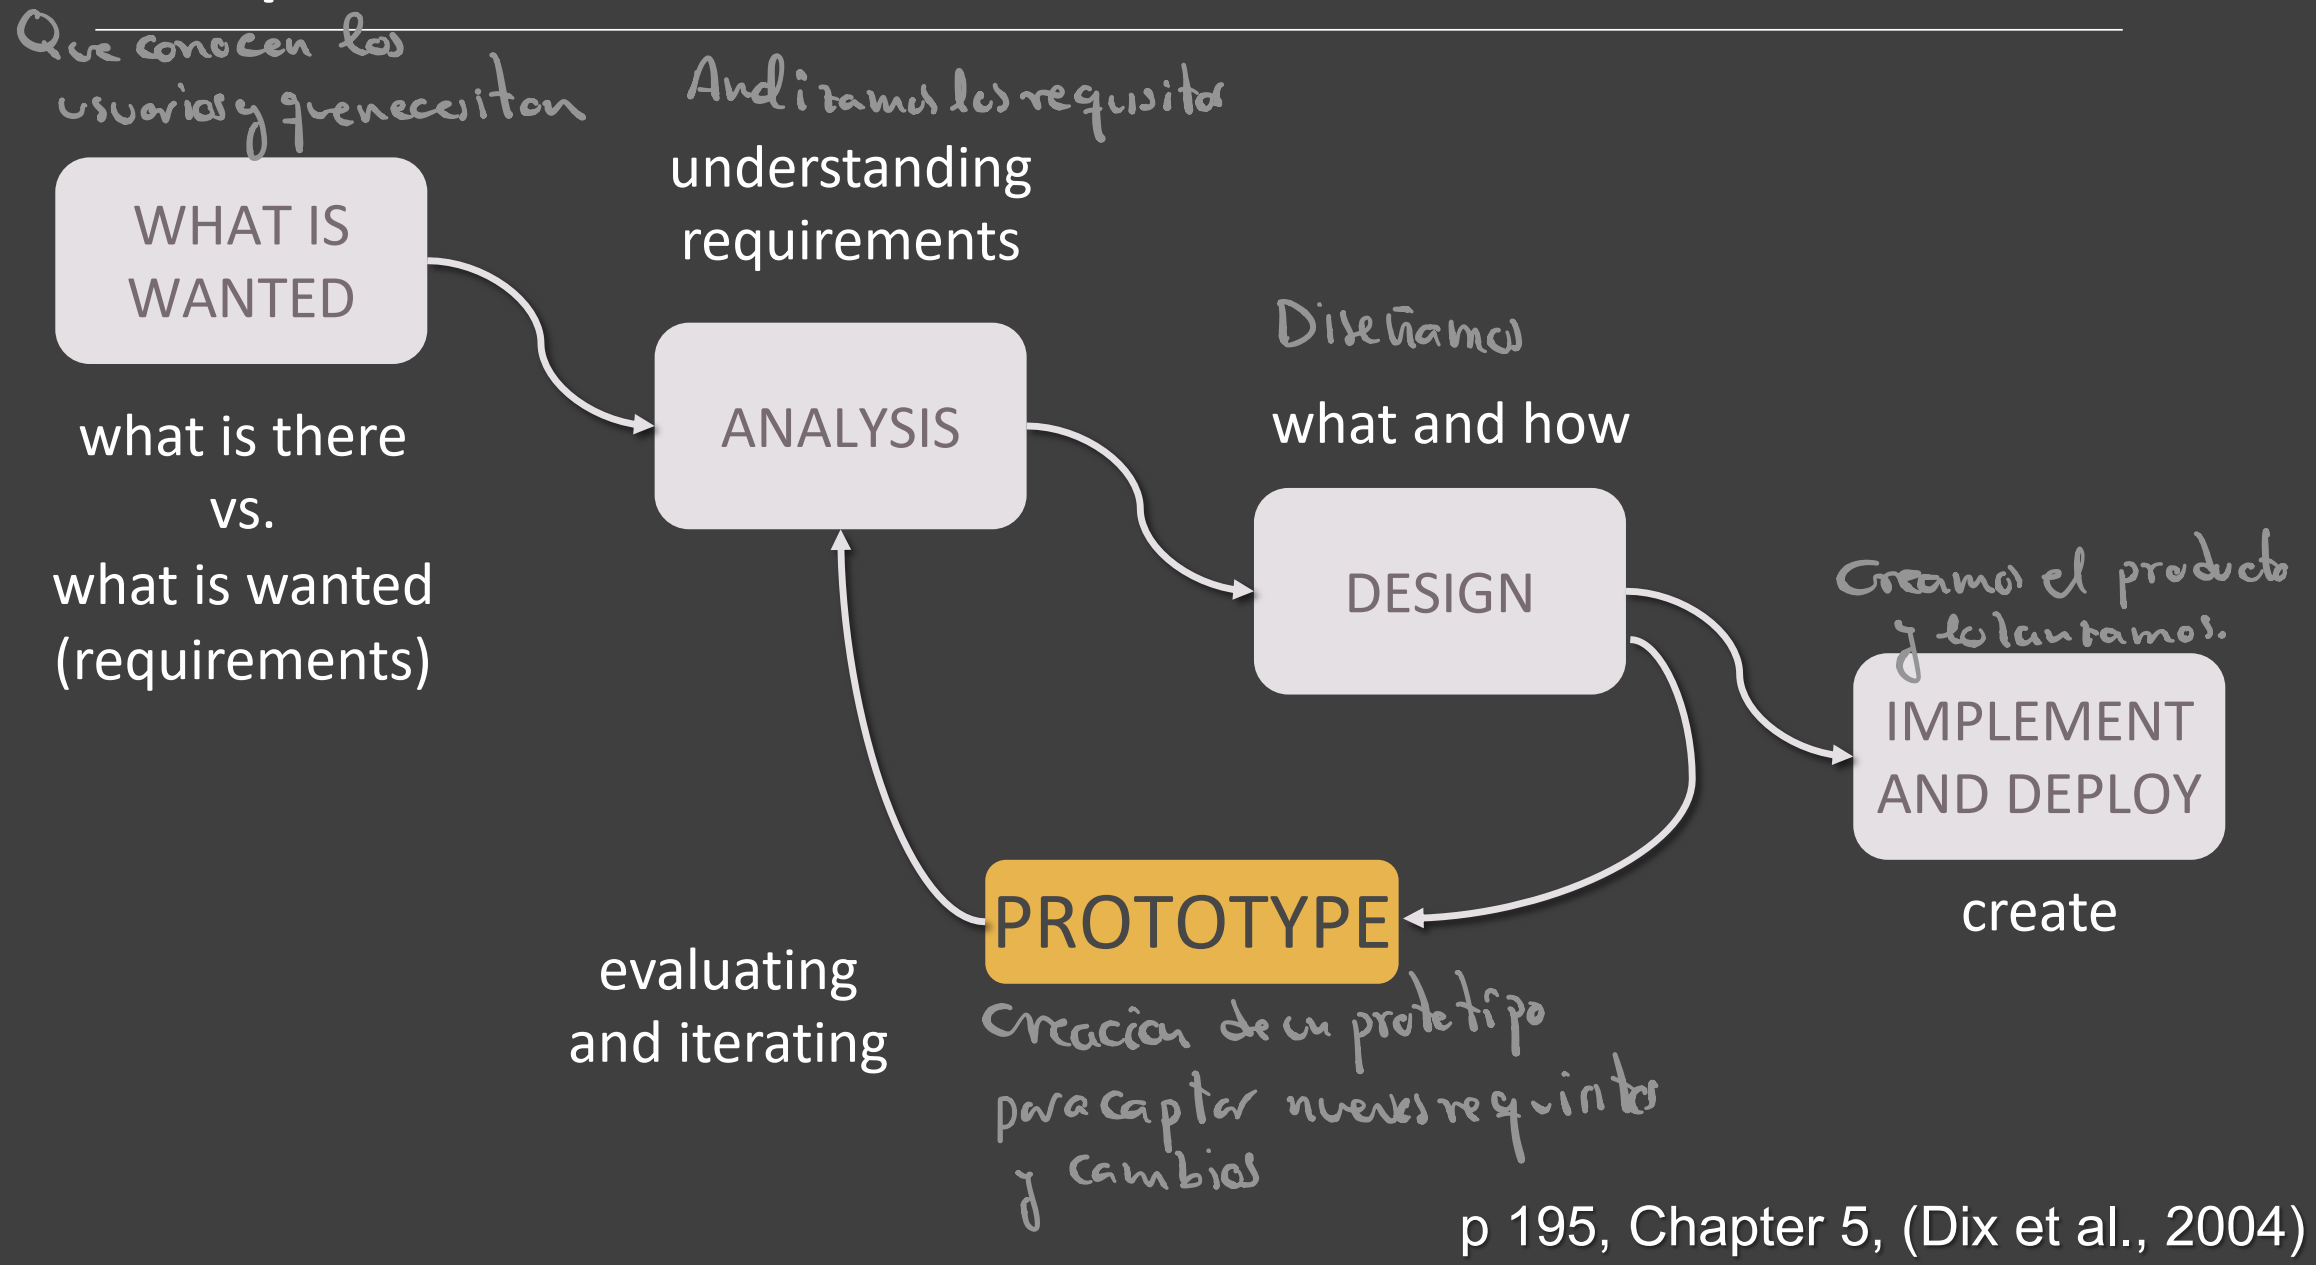
\includegraphics[scale=.18]{Untitled 3.png}}
\end{figure}
\subsubsection{What is wanted}
Que conocen los usuarios y que necesitan.

    \begin{itemize}
    
    \item
      Conocer al usuario:

      \begin{itemize}
      
      \item
        Los usuarios o stakeholders son aquellos que lo van a usar o
        están afectados por el sistema.
      \item
        Es importante hablar con ellos y observarlos, hay que
        identificarlos y crear perfiles de usuarios del sistema. Se
        pueden definir personas.
      \item
        Persona: Representación de un usuario ficticio típico,
        descripción detallada de un usuario típico del sistema,
        incluyendo objetivos, capacidades, actitudes, tareas y contexto.
      \end{itemize}
    \item
      Métodos etnográficos:

      \begin{itemize}
      
      \item
        Cada acción está relacionada con el sitio, el contexto social y
        el momento en el que se lleva a cabo.
      \item
        Se observa la interacción entre las personas y entre las
        personas y el contexto en el que se encuentran para tomar nota
        de la información más relevante y útil para el desarrollo del
        sistema.
      \item
        El contexto puede estar relacionada con una situación particular.
      \end{itemize}
    \end{itemize}
\subsubsection{Analysis}
	Analizamos los requisitos.

    \begin{itemize}
    
    \item
      Conocer al usuario:

      \begin{itemize}
      
      \item
        Analizar los resultados obtenidos de la observación de los
        usuarios y de las entrevistas.
      \item
        Identificar los factores más relevantes de la fase de diseño.
      \item
        Analizar como los usuarios llevan a cabo las tareas con sistemas
        similares.
      \item
        Utilizar modelos cognitivos para representar la interacción
        entre los usuarios y los sistemas.
      \end{itemize}
    \end{itemize}
\subsubsection{Design}
	Como y el que.

    \begin{itemize}
    
    \item
      Diseño centrado en el usuario:

      \begin{enumerate}
      \def\labelenumi{\arabic{enumi}.}
      
      \item
        El diseñador se hace una idea de cuáles son las necesidades del
        usuario y las tareas.
      \item
        El diseñador traslada sus ideas al diseño del sistema.
      \item
        El usuario interpreta la interfaz del sistema y se hace una idea
        propia de cómo funciona.
      \end{enumerate}

      \begin{itemize}
      
      \item
        Cuando la idea no corresponde con la del diseñador, se rediseña
        o se frustrará.
      \item
        El usuario es el centro del proceso de diseño.
      \item
        El usuario tiene que entender la imagen del sistema definida por
        el diseñador.

        \begin{itemize}
        \item
          User requirements: Entender y especificar el contexto de uso.

          \begin{itemize}
          
          \item
            Identificar a los usuarios a los que se dirige el producto,
            para que lo usaran y en qué condiciones.
          \end{itemize}
        \item
          Analysis: Especificar requisitos.

          \begin{itemize}
          
          \item
            Identificar los objetivos del usuario que el producto deberá
            satisfacer.
          \item
            Se llevarán a cabo actividades que involucran el usuario,
            como entrevistar, grupos focales, etc.
          \end{itemize}
        \item
          Design: Producir varias soluciones de diseño a través de
          prototipos.

          \begin{itemize}
          
          \item
            Los prototipos se podrán diseñar con varios niveles de
            detalles dependientes de las necesidades del diseñador.
          \end{itemize}
        \item
          Evaluation: La evolución es la fase más importante del
          proceso.

          \begin{itemize}
          
          \item
            Se validan los prototipos para comprobar si satisfacen los
            requisitos o por el contrario se detectan problemas de
            usabilidad.
          \end{itemize}
        \end{itemize}
      \end{itemize}
    \end{itemize}

\subsubsection{Prototype}
Creación de un prototipo para captar nuevos requisitos y
    cambios.

    \begin{itemize}
    
    \item
      ¿Qué es?

      \begin{itemize}
      
      \item
        Conjunto de bocetos de las pantallas.
      \item
        Storyboard, escenas en estilo animado.
      \item
        Presentación PowerPoint
      \item
        Video de la simulación.
      \item
        Objeto físico de algún material específico.
      \item
        Mock-up en papel.
      \item
        Sistema con un conjunto limitado de funcionalidades.
      \end{itemize}
    \item
      ¿Por qué?

      \begin{itemize}
      
      \item
        Evaluar la idea del diseñador y recibir feedback.
      \item
        Para que los stakeholder vean, toquen e interactúen.
      \item
        Para tomar decisiones sobre el diseño más fácilmente.
      \item
        Testear ideas.
      \end{itemize}
    \item
      The Rapid Prototyping Process: Proceso en tres fases para
      construir y mejorar prototipos rápidamente.

      \begin{enumerate}
      \def\labelenumi{\arabic{enumi}.}
      
      \item
        Definir el prototipo especificando cualquier interacción o
        funcionalidad se quiere añadir.
      \item
        Evaluar el prototipo con o sin usuarios dependiendo del contexto
        y de la fase de diseño en, aunque nos encontramos.
      \item
        Redefinir el prototipo. Se pueden ir añadiendo más
        funcionalidades o más detalles.
      \end{enumerate}

      \begin{itemize}
      
      \item
        Se itera el proceso hasta llegar a una versión adecuada.
      \end{itemize}
	  \pagebreak
    \item
      Según cualidades:

      \begin{itemize}
      
      \item
        Representación - forma física.
      \item
        Fidelidad -- precisión o el nivel de detalle y de realismo.

        \begin{itemize}
        
        \item
          Fidelidad funcional: Prototipos horizontales, mayor número de
          funcionalidades, pero bajo nivel de detalle.
        \item
          Fidelidad visual: Prototipos verticales, menor número de
          funcionalidades, pero alto nivel de detalle.
        \end{itemize}

        \begin{enumerate}
        \def\labelenumi{\arabic{enumi}.}
        
        \item
          Low visual + low functionality: Prototipos rápidos fáciles de
          realizar que se pueden usar durante las primeras fases del
          proceso de diseño para ir definiendo las funcionalidades y los
          requisitos del sistema.
        \item
          Low visual + high functionality: Wireframes que se realizan
          generalmente con algún tipo de herramienta específica para
          interacciones de bajo nivel. Permiten evaluar la usabilidad
          del sistema con y sin usuario y hacer pruebas de concepto.
        \item
          High visual + low functionality: Mock-ups a los que se añade
          alguna interacción más avanzada. Se pueden usar animaciones
          para simular el cambio entre funcionalidades o cambio de
          pantalla. Sirve para evaluar el flujo del sistema.
        \item
          High visual + high functionality: Realizados durante el último
          paso antes del desarrollo del producto final. Se usan para
          evaluar la usabilidad de las funciones y de la interfaz tal y
          como será en el producto final.
        \end{enumerate}
      \item
        Interacción -- hasta qué punto el usuario puede interactuar con
        el prototipo.
      \item
        Evolución -- el ciclo de vida del prototipo.
      \end{itemize}
    \end{itemize}

\subsubsection{Implement and deploy}
Creamos el producto y lo lanzamos.

  
\pagebreak
\section{Accesibilidad}
  Que se pueda utilizar por cualquier persona a pesar de limitaciones
  físicas, psíquicas o del contexto. Se trata de diseñar para todos los
  usuarios posibles.

  Los sistemas usables tienen como objetivo el satisfacer a personas con
  diferentes características, necesidades y requisitos.

  \begin{itemize}
  
  \item
    Personas con discapacidad
  \item
    Personas de todas las edades
  \item
    Personas con diferentes habilidades y niveles de experiencia
  \item
    Personas de todo el mundo que hablan idiomas distintos
  \item
    Personas de diferentes culturas
  \end{itemize}

  Tienen que tener en cuenta también el contexto en los que se utilizan,
  comunicación, trabajo, salud, cultura, etc.

  Tecnología adaptativa: Productos o dispositivos para mejorar o
  aumentar las capacidades funcionales de las personas con algún tipo de
  discapacidad.

  \begin{itemize}
  
  \item
    Teclado adaptativo: Las teclas son más grandes que las de un teclado
    normal y tienen colores alegres.

    \begin{itemize}
    
    \item
      Disposición clara y amigable para que los niños se familiaricen
      con el ordenador.
    \item
      Útil para personas con discapacidad de aprendizaje o motora.
    \end{itemize}
  \item
    Footmouse -- Ratón de pie: Un ratón que se puede utilizar con los
    pies, para mover el cursor y hacer clic.
  \item
    Lectores de pantalla, pantallas Braille para ciegos, magnificadores
    de pantalla, dispositivos de entrada y salida para personas con
    problemas de movimiento.
  \end{itemize}
\pagebreak
  Diseño universal: Diseño de productos usables para todos, sin
  necesidad de ser adaptados o mejorados, no necesita dispositivos
  adaptativos.

  \begin{itemize}
  
  \item
    Mejora la vida de todos, beneficios para todas las edades y
    habilidades.
  \item
    Siete principios para el diseño universal:

    \begin{enumerate}
    \def\labelenumi{\arabic{enumi}.}
    
    \item
      Uso equitativo: Diseño útil para todas las personas.
    \item
      Uso flexible: El diseño se acomoda a un amplio rango de
      preferencias.
    \item
      Uso simple e intuitivo: El uso del diseño es fácil de entender,
      sin importar la experiencia.
    \item
      Información perceptible: El diseño transmite la información
      necesaria de forma efectiva al usuario.
    \item
      Tolerancia al error: El diseño minimiza riesgos y consecuencias de
      acciones involuntarias o accidentales.
    \item
      Mínimo esfuerzo físico: El diseño puede ser usado cómodamente y
      eficientemente.
    \item
      Tamaño de aproximación y uso: Tamaño y espacio adecuado para el
      alcance, manipulación y uso, independientemente del tamaño
      corporal, postura o movilidad del usuario.
    \end{enumerate}
  \end{itemize}

  Design 4 All

  \begin{itemize}
  
  \item
    Incluye el diseño accesible, diseño inclusivo, diseño sin barreras,
    diseño universal.
  \item
    Aplica principios, métodos y herramientas específicas.
  \item
    Desarrolla servicios y productos IT accesibles y usables para todos.
    No se necesitan adaptaciones a posteriori.
  \item
    La comunicación entre los usuarios, los stakeholders y los equipos
    de diseños es fundamental.

    \begin{itemize}
    
    \item
      Entrevistas, cuestionarios, prototipos, observación, etc.
    \end{itemize}
  \end{itemize}

  Calidades del diseño

  \begin{itemize}
  
  \item
    Accesibilidad: Los productos tienen que tener en cuenta habilidades
    limitadas y específicas.
  \item
    Usabilidad: Los productos tienen que cumplir con los requisitos y
    las necesidades de los usuarios.
  \end{itemize}

  Factores de diversidad:

  \begin{itemize}
  
  \item
    Diversidad de Usuarios:

    \begin{itemize}
    
    \item
      Discapacidad: Grupos de usuarios con habilidades y necesidades
      comunes para adaptar el diseño de la interacción.

      \begin{itemize}
      
      \item
        Percepción -- discapacidad auditiva y visual.
      \item
        Movimiento -- discapacidad física.
      \item
        Cognición -- habilidades de la mente humana de procesar
        información, pensar, recordad, razonar y tomar decisiones.
      \end{itemize}
    \item
      Edad: Perciben y procesan la información de forma distinta
      dependiendo de su edad. Puede ayudar al diseñador a tomar
      decisiones sobre cómo presentar la información.

      \begin{itemize}
      
      \item
        Niños.
      \item
        Mayores y ancianos.
      \end{itemize}
    \item
      Experiencia: Dependen también de las experiencias y los
      conocimientos previos que tiene el usuario con la tecnología.

      \begin{itemize}
      
      \item
        Opciones accesibles: Menú de ayuda, documentación más detallada,
        uso de etiquetas e iconos.
      \end{itemize}
    \item
      Cultura: Incluir detalles relacionados con la cultura del usuario,
      para hacer un sistema más inclusivo y tolerante.

      \begin{itemize}
      
      \item
        Barreras del idioma.
      \item
        Diferencias culturales al interpretar símbolos, colores,
        gestos\ldots{}
      \end{itemize}
    \item
      Social: Condición social y las oportunidades educativas pueden
      crear barreras de acceso a la tecnología.
    \end{itemize}
  \item
    Diversidad Tecnológica: El entorno puede representar un impedimento
    a la hora de utilizar un sistema. El usuario podría resultar
    temporalmente discapacitado.

    \begin{itemize}
    
    \item
      Web Accessibility: Garantizar que personas con discapacidad u
      otros grupos de usuarios vulnerables puedan acceder, entender,
      navegar e interpretar con el contenido disponible en internet.
      También para que puedan contribuir publicando nuevo contenido.
    \item
      Guías Web de Accesibilidad:

      \begin{itemize}
      
      \item
        WCAG: Hacer todo el contenido web accesible. Basada en una
        amplia experiencia de expertos en el dominio.

        \begin{itemize}
        
        \item
          Son principios generales de diseño accesible.
        \item
          3 niveles: A, AA y AAA.
        \end{itemize}
      \item
        WAI-ARIA: Hacer el contenido dinámico y los controles avanzados
        de la interfaz de usuario accesibles. Los elementos web
        avanzados podrían afectar la accesibilidad.
      \item
        Surgen limitaciones en la aplicación de las guías: Necesitan un
        entrenamiento extensivo y lleva tiempo aplicarlas.
      \item
        Hay herramientas semiautomáticas para comprobar archivos HTML.
      \end{itemize}
    \end{itemize}
  \end{itemize}

  Técnicas de interacción:

  \begin{itemize}
  
  \item
    Voz: Manos del usuario están ocupadas o no puede utilizar ni el
    teclado ni el ratón.

    \begin{itemize}
    
    \item
      Sistema de salida de voz.
    \item
      Sistemas de reconocimiento de voz.
    \item
      Sistemas de diálogo hablado, tanto entrada como salida.
    \end{itemize}
  \item
    Háptica: Cooperación entre sensores en la piel y sensores en los
    músculos. Exploración a través de las manos para recopilar
    información a través del tacto activo.

    \begin{itemize}
    
    \item
      Tacto remoto, experiencia de un objeto distante.
    \item
      Leer textos, equivalencia táctil de letras visuales.
    \item
      Manipulación háptica de objetos.
    \end{itemize}
  \item
    Interacción basada en escaneo: Interacción a través de
    interruptores, el marcador de enfoque escanea la interfaz para
    resaltar objetos interactivos secuencialmente.

    \begin{itemize}
    
    \item
      Es lento, pero útil.
    \item
      Se puede activar mediante diferentes modalidades.

      \begin{itemize}
      
      \item
        Mano, dedo, pie, lengua, cabeza, aliento, ojo, teclado, ratón.
      \end{itemize}
    \item
      Para usuarios con dificultades para usar dispositivos de entrada
      clásicos.
    \end{itemize}
  \item
    Eye tracking: Usar la mirada para comunicarse. Cuando la mirada es
    la única opción de comunicación disponible, se utiliza para
    seleccionar elementos.

    \begin{itemize}
    
    \item
      Problemas: Movimientos oculares involuntarios o demasiado rápidos.
    \item
      No se puede revisar lo que está escribiendo al mismo tiempo que se
      está escribiendo.
    \item
      Aproximadamente 10 palabras por minuto.
    \end{itemize}
	\pagebreak
  \item
    Monitorización de gesto y cabeza: Los gestos como características
    importantes de las expresiones humanas.

    \begin{itemize}
    
    \item
      Varios enfoques para el reconocimiento de gestos.
    \item
      Interactuar mediante gestos.
    \item
      No solo gestos con las manos, sino también con la cabeza y el
      cuerpo.
    \end{itemize}
  \item
    Interfaces cerebrales: Sistemas de comunicación en tiempo real para
    enviar mensajes usando bioseñales del cerebro.

    \begin{itemize}
    
    \item
      Usuarios con partes de su cerebro activas, pero si ningún otro
      medio de comunicación.
    \item
      Dos tipos:

      \begin{itemize}
      
      \item
        Invasivos: Sondas dentro del cerebro.
      \item
        No invasivo: Electrodos colocados externamente.
      \end{itemize}
    \item
      Los biopotenciales son señales eléctricas obtenidas del cuerpo,
      cada una tiene sus propias características.
    \end{itemize}
  \item
    Lenguaje de signos: Usuario que por determinadas circunstancias
    utiliza un lenguaje de señas para comunicarse.

    \begin{itemize}
    
    \item
      Sistemas de traducción automática de texto en ingles a animaciones
      en lenguaje de signos.
    \item
      Introducir comandos en un sistema informático usando lenguaje de
      signos y, como resultado obtener como salida, texto, voz o lengua
      de signos.
    \end{itemize}
  \item
    Interfaces multimodales: Dos o más modos de entrada.

    \begin{itemize}
    
    \item
      Multisensorial: Múltiples modalidades sensoriales.
    \item
      Multicanal: varios canales para la misma o diferentes modalidades.
    \item
      Multitarea: Varias tareas al mismo tiempo.
    \item
      Multiforma: Las mismas tareas de formas alternativas.
    \end{itemize}
  \end{itemize}

\chapter{TEMA 3 - Diseño Web}
\section{Diseño Web}

Evolución de la web: Hoy en día es un universo de aplicaciones y
páginas web interconectadas llenas de contenido multimedia e
interactivo.

Sitio web: Colección de páginas web relacionadas y comunes a un
dominio de Internet o subdominio de la World Wide Web.

\subsection{Principios básicos}


    Debe satisfacer las necesidades del usuario.

    Evitar la navegación lineal: Permite navegar sin seguir u orden
    estricto, moverse de una página a otra sin orden.
  
    El usuario debe saber en todo momento donde se encuentra, que
    puede hacer y como desplazarse a otros contenidos.

    Facilitar la búsqueda de contenidos.

    
\subsection{Aspectos a considerar en el diseño del sitio:}

Estructura de la información.
\begin{figure}[H]
  \ffigbox[\FBwidth]
  {\caption{Estrucutra de una Web}}
  {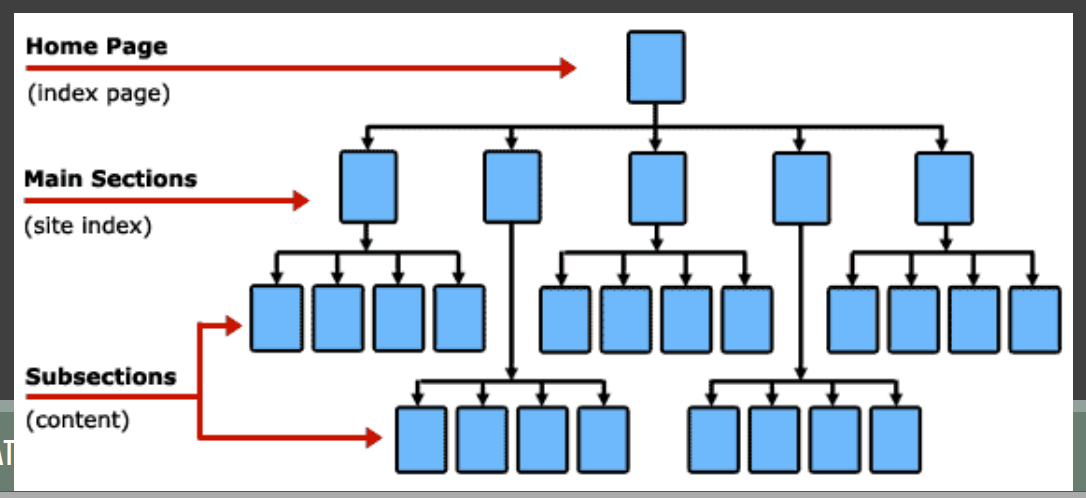
\includegraphics[scale=.3]{Untitled 6.png}}
\end{figure}
\begin{itemize}
  \item
    Centrada en las tareas del usuario.
  \item
    Anteponer anchura frente a profundidad, poder ver las
    principales tareas primero, y si se quiere más información se
    profundiza.
    \begin{itemize}
      \item
        3 es un buen nivel de profundidad.
    \end{itemize}
  \item
    Agrupamientos lógicos de contenidos.
  \item
    Un objetivo/ dos tareas: Que haya dos maneras de llegar a los
    objetivos por si se ha saltado uno de ellos.
  \item Secciones:
    \begin{itemize}
      \item Página principal -- Homepage:
        \begin{itemize}
          \item Función: Indicar al usuario donde esta y funciones del sitio
            web.
            \begin{itemize}
              \item
                Información a mostrar:

                Logo de la organización.

                Nombre del sitio web.

                Introducción al sitio.

                Enlaces a las páginas principales del sitio.

                Resumen de los contenidos principales del sitio.

                Información de contacto / Políticas de uso / Condiciones
                de acceso.

                Resumen de últimas noticias / promociones / cambios en
                el sitio.
            \end{itemize}
        \end{itemize}
      \item Secciones principales
        \begin{itemize}
          \item
            Mantener logo y nombre (reducir tamaño)
          \item
            Enlace a la página principal
          \item
            Elementos de ayuda a la navegación
          \item
            Enlaces al resto de secciones principales
        \end{itemize}
      \item Subsecciones
        \begin{itemize}
          \item
            Mantener logo y nombre del sitio web
          \item
            Indicar con claridad la sección principal a la que pertenece
          \item
            Indicar la localización con respecto a la estructura del
            sitio (¿dónde estoy?)
          \item
            Centrarse en el contenido más que en la navegación
          \item
            Facilitar la ejecución de acciones
        \end{itemize}
    \end{itemize}
\end{itemize}

      
Navegación por el sitio.

\begin{itemize}
    \item Navegación: Capacidad de moverse por el sitio web para conseguir
      los objetivos del usuario.
    \item Es la forma básica de recogida de información en los sitios web.
      \begin{itemize}
        \item Se puede hacer mediante: Enlaces u otro tipo de herramienta.
      \end{itemize}
      \pagebreak
    \item Estoy:
      \vspace{-0.5cm}
      \begin{itemize}
      
        \item
          En la web como un todo, título de la página, breve
          introducción\ldots{}
        \item
          Respecto al propio sitio web, opción de menú destacada, migas
          de pan\ldots{}
      \end{itemize}
    \item He estado:
      \vspace{-0.5cm}
      \begin{itemize}
      
        \item
          Basándose en el navegador, botón atrás, historial\ldots{}
        \item
          Basándose en el diseño del sitio web, migas de pan,
          cookies\ldots{}
      \end{itemize}
    \item Puedo ir:
      \vspace{-0.5cm}
      \begin{itemize}
      
        \item
          Enlace y ayudas a la navegación
      \end{itemize}
    \item Tipos de enlaces

      \begin{itemize}
      
        \item
          Estructurales

          \begin{itemize}
          
            \item
              Enlaces a otras páginas (del mismo sitio)
            \item
              Establecen la estructura del sitio
          \end{itemize}
        \item
          Asociativos

          \begin{itemize}
          
            \item
              Enlaces a otros contenidos de la propia página
            \item
              Facilita la navegación en textos extensos
          \end{itemize}
        \item
          Embebidos

          \begin{itemize}
          
            \item
              Enlaces a otras páginas o, incluso, otros sitios web
            \item
              Información adicional
          \end{itemize}
      \end{itemize}
    \item Diseño de enlaces

      \begin{itemize}
      
        \item
          Enlaces textuales: Lo que los identifica es el color, pero son
          una palabra o frase en el contenido.

          \begin{itemize}
          
            \item
              Color: Asegura la consistencia y los distingue del resto de
              contenido.
            \item
              Nombre: texto significativo y explicativo.
            \item
              Incluye ayudas contextuales.
          \end{itemize}
        \item
          Enlaces no textuales: No se trata de texto en color, sino que
          es otro elemento como:

          \begin{itemize}
          
            \item
              Botones
            \item
              Gráficos
            \item
              Listas desplegables
            \item
              Imágenes
            \item
              Mapa en el que se puede acceder a secciones del lugar.
            \item
              Migas de pan- bread crumbs.
          \end{itemize}
      \end{itemize}
      \pagebreak
    \item Ayudas a la navegación - Visita guiada
      \begin{itemize}
        \item Visita guiada
        \item Mapas del Sitio
        \item Directorios
        \item Volver atrás (migas de pan): Ir a secciones superiores en la jerarquía.
        \item Opciones de ayuda: Dar más información de un contenido/termino.
        \item Opciones de búsqueda: Barra de búsqueda.
        \item Uso de metáforas: Por asociación a algo que existe en el mundo real
      \end{itemize}
    \item Problema

    \begin{itemize}

      \item
      No indicar al usuario donde se encuentra

        \begin{itemize}
          \item Páginas en blanco
          \item
            Uso del mismo título en varias páginas 
          \item Inconsistencia entre
            nombre del enlace y título de la página asociada.
        \end{itemize}
      \item
      No indicar al usuario el camino 

        \begin{itemize}
          \item Enlaces autorreferenciados
          \item
            Exceso de enlaces embebidos. 
          \item Profundidad excesiva/ Demasiados
            niveles de búsqueda.
        \end{itemize}
      \item No facilitar búsqueda adecuada 

        \begin{itemize}
          \item Pobre navegación entre los
      resultados.
          \item
            Resultados numerosos o poco relacionados.
        \end{itemize}
    \end{itemize}
\end{itemize}

Interacción.

\subsection{Diseño detallado del sitio}
\subsubsection{Páginas}
Cada uno de los documentos o espacios de interacción que conforman un sitio
  web. 

Principios básicos: 
\begin{itemize}
  \item Dar preponderancia al contenido frente a
  la estética o la navegación
  \item Separar contenido de presentación
  \item Independencia de plataforma
  \item Asegurar la consistencia
\end{itemize}

Layout
\begin{itemize}
  \item Crear agrupaciones intuitivas, de contenidos y de acciones.
  \item Destacar los componentes más importantes.
  \item  Hacer los controles visibles.
  \item Equilibrio entre estética y usabilidad.
  \item Usar el espacio en blanco a
  fin de facilitar la exploración de contenidos. 
\end{itemize}

Scrolling: 
\begin{itemize}
  \item Los contenidos más importantes por encima del tamaño de página.
  \item Páginas cortas para la página principal, navegación o de acceso inmediato.
  \item El contenido por encima del tamaño normal debe animar o mostrar la
  utilidad de hacer scroll.
  \item Reducir el scroll vertical a un par de
  desplazamientos.
  \item Evitar siempre el scroll horizontal.
\end{itemize}


\subsubsection{Widgets}
Componente software concebido para proveer información visual y facilitar una interacción determinada.

Proceso de diseño basado en widgets
\begin{itemize}
  \item Estructurar la interacción.
  \item Controlar la interacción.
  \item Introducir información.
\end{itemize}					
\pagebreak
\subsubsection{Contenidos}
Conjunto de textos, imágenes, videos y, en general, elementos multimedia que determinan la información proporcionada por un sitio web.

Principios básicos:
\begin{itemize}
  \item Reducir el tiempo de descarga, inferior a 1s y máximo 10 s.
  \item Facilitar la exploración frente a búsqueda exhaustiva.
  \item Respetar los principios del diseño universal.
  \item Evitar el uso de sonidos y locuciones siempre que no sean imprescindibles para dar feedback.
\end{itemize}
		
Texto:
\begin{itemize}
  \item Minimizar la extensión del texto, el necesario no poner información superflua.
  \begin{itemize}
    \item Eliminar párrafos introductorios.
    \item No incluir información superflua o de autobombo.
    \item Utilizar tablas y enumeraciones para organizar la información.
  \end{itemize}
  
  \item Ayudar al usuario a explorar la información.
  \begin{itemize}
    \item Incluir títulos en todas las páginas.
    \item Utilizar titulares para estructurar la información.
    \item Separa bloques de información extensos en secciones.
    \item Destacar la información de interés o más relevantes.
  \end{itemize}
 
  \item No utilizar jerga.
\end{itemize}
			


Utilidad vs Usabilidad
\begin{itemize}
  \item
  Relacionadas, pero no son lo mismo.
\item
  Utilidad se refiere únicamente al uso que se hace de un sistema.
\item
  Usabilidad incluye no solo la usabilidad, sino también la
  eficiencia, seguridad, memorabilidad, capacidad de aprendizaje y
  satisfacción.
\end{itemize}
\pagebreak

    Recomendaciones para mejorar la utilidad

    \begin{itemize}
    
    \item
      El usuario puede realizar la tarea eficientemente

      \begin{itemize}
      
      \item
        Sabe cómo llevarla a cabo.
      \item
        La descomposición de la tarea en acciones y su secuenciación son
        adecuadas.
      \item
        Reduce la ansiedad, mostrando el estado de la tarea.
      \item
        Se le estimula para completar la tarea.
      \item
        No se producen errores, y si se producen, tienen una solución
        muy sencilla.
      \item
        No se producen retardos innecesarios.
      \item
        Se eliminan las distracciones.
      \end{itemize}
    \item
      La utilidad de la herramienta (web o Sistema interactivo) es
      evidente

      \begin{itemize}
      
      \item
        A primera vista el usuario debe saber que puede hacer.
      \item
        Menús con las opciones principales.
      \end{itemize}
    \item
      Mantener el sistema accesible

      \begin{itemize}
      
      \item
        Siempre debe dar una respuesta rápida.
      \item
        Evitar sitios/páginas en construcción o que no redirigen al
        nuevo sitio web.
      \end{itemize}
    \item
      Eliminar cualquier tipo de reiteración, incertidumbre o sorpresa
    \item
      Los contenidos multimedia no deben disminuir la utilidad de la
      aplicación

      \begin{itemize}
      
      \item
        Los elementos multimedia ocupan mucho espacio y aumentan el
        tiempo de carga de la página
      \item
        Se genera incertidumbre y aburrimiento en el usuario.
        Soluciones:

        \begin{itemize}
        
        \item
          No embeber el material multimedia, hacerlo descargable
        \item
          Incluir un enlace al material multimedia o un m-icon
        \end{itemize}
      \item
        Si se requiere alguna aplicación externa para acceder a algún
        tipo de contenido:

        \begin{itemize}
        
        \item
          Advertirlo en la interfaz
        \item
          Proporcionar un medio de acceder a ese software
        \end{itemize}
      \end{itemize}
    \end{itemize}
    \pagebreak
    Recomendaciones para mejorar la usabilidad

    \begin{itemize}
    
    \item
      Orientar el diseño a los potenciales usuarios (características y
      necesidades).

      \begin{itemize}
      \item
        El diseño de nuestra web debe estar orientado al usuario.
      \item
        Hay que considerar las características y necesidades de los
        usuarios.

        \begin{itemize}
        
        \item
          Edad, idioma, objetivos, requisitos de eficiencia o
          familiaridad.
        \end{itemize}
        \item Diseño para todos: La usabilidad ha de garantizarse para el máximo
  número de usuarios posibles, si necesidad de adaptación.
      \end{itemize}

    
      

\item Potenciar la legalidad frente a la vistosidad
\begin{itemize}
  \item Combinación de elementos multimedia
  \begin{itemize}
    \item Evitar animaciones innecesarias y gráficos complejos.
    \item Evitar elementos simultáneos que demanden la atención.
  \end{itemize}
   
    \item Considerar la capacidad de procesamiento de la información.
\item El texto
\item Las imágenes
\item Las locuciones, primar la claridad.
\item Las plantillas para organizar los elementos y crear composiciones de una forma armónica.
\item Utilizar colores con alto contraste entre el texto y el fondo.
\item El texto debe ser estático, sin elementos parpadeantes o en movimiento.
\item Extensión de línea: unos 60 características.
\item Tipo de letra:
\begin{itemize}
  \item Fuente de letra que facilite la lectura (Arial, Times, Sans Serif).
  \item Tamaño de fuente de letra adecuado (11-13 puntos).
  \item Adecuar el espacio entre líneas.
  \item No utilizar mayúsculas.
\end{itemize}
    
  \item Justificar el texto a la izquierda.
  \item El fondo no debe dificultad la lectura.
  \item  Calidad de la imagen vs. cantidad de espacio
  \begin{itemize}
    \item Menor calidad de imagen.
    \item Imágenes de mejor calidad bajo demanda.
    \item Debería verse completa en configuraciones estándar.
    \item Tener en cuenta el tamaño si queremos que se pueda imprimir.
  \end{itemize}
  \begin{figure}[H]
    \ffigbox[\FBwidth]
    {\caption{Tipos de colores}}
    {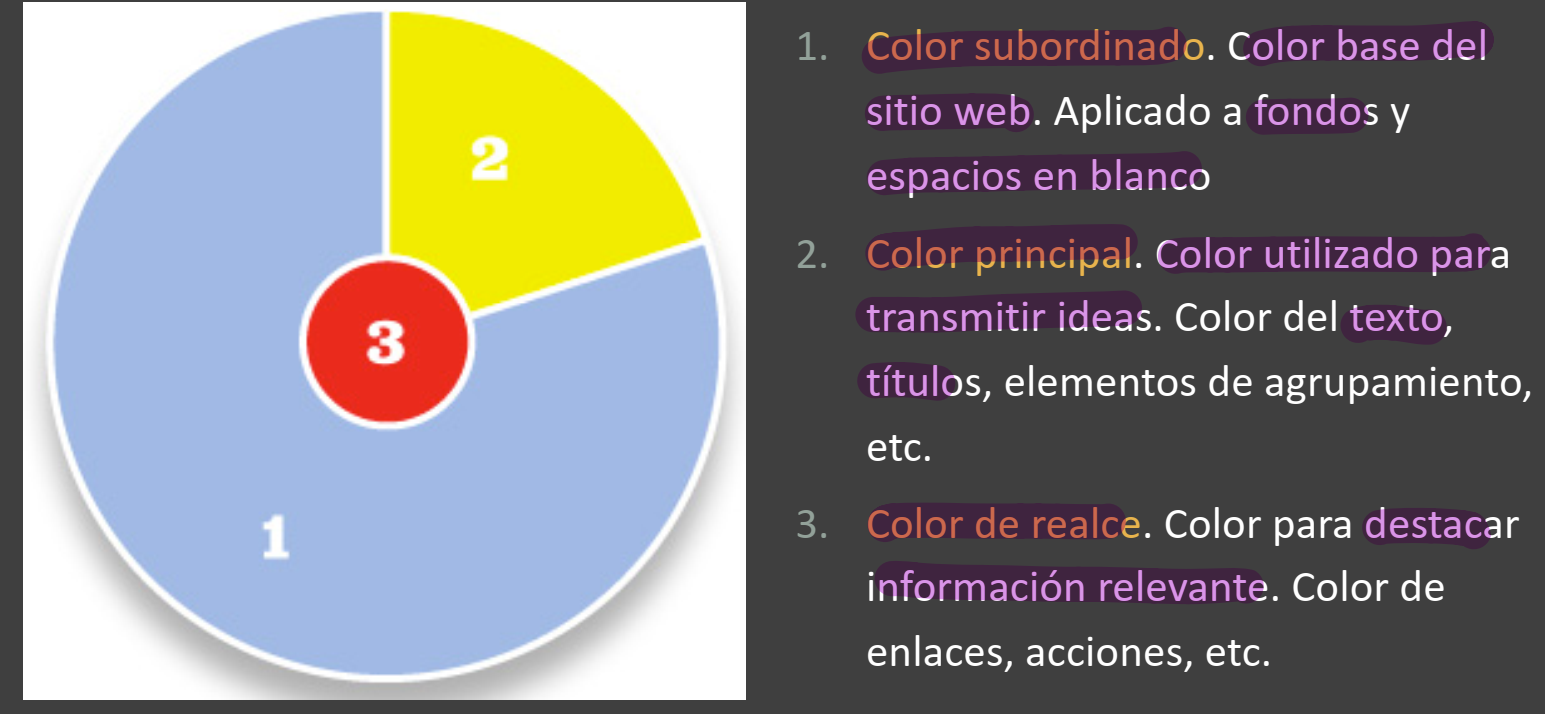
\includegraphics[scale=.25]{Untitled 16.png}}
  \end{figure}
\end{itemize}
  

    
    \item
      Mantener la consistencia

      \begin{itemize}
      
      \item
        Debe hacerse un uso semántico del color y de otros recursos
        audiovisuales.
      \item
        Utilizar los nombres para referirse a las mismas cosas.
      \item
        Mismas funcionalidades deben activarse siempre del mismo modo y
        producir el mismo tipo de resultados.
      \item
        Iconos deben ser concretos y familiares, visual y
        conceptualmente distintos.
      \item
        Utilizar pocos iconos y significativos
      \end{itemize}
    \item
      Las funciones y los datos del sistema tienen que ser tangibles.

      \begin{itemize}
      
      \item
        La estructura de la información se puede hacer explícita:

        \begin{itemize}
        
        \item
          Páginas autocontenidas.
        \item
          Buen uso de los enlaces.
        \item
          Usando los elementos multimedia para realzar el contenido de
          las páginas para que sean más fácilmente identificables.
        \item
          Empleando herramientas de navegación que den una idea de la
          estructura global/parcial.
        \end{itemize}
      \item
        Las metáforas son simulaciones de entorno ya conocidas por el
        usuario
      
        \begin{itemize}
          \item
          El escritorio, el libro electrónico, el carrito de
          compra \ldots{}
  
        \item
          Siguen patrones de uso reconocibles por los usuarios.

          \item
        Incrementan la tangibilidad.
        \end{itemize}
      
      \end{itemize}
    \end{itemize}
\pagebreak
\section{Principio de diseño Web}


    Son abstracciones generalizables que tienen como objetivo orientar a
    los diseñadores. Procesen de la teoría, la experiencia y el sentido
    común. No existe una regla de oro.

\subsection{Tipos de artefactos:}

\subsubsection{Heurísticas}
	  Abstracciones generalizables basadas en la
      experiencia, el sentido común o la teoría.

      \begin{itemize}
      
      \item
        Heurísticas de Schneiderman: No hace falta sabérselas.
      \item
        Heurísticas de Nielsen y Molich: No hace falta sabérselas.
      \item
        Heurísticas de Nielsen: Es en las que nos centraremos.

        \begin{itemize}
        
        \item
          Visibilidad del estado del sistema: Barras de progreso o
          animaciones de carga.
        \item
          Coincidencia entre el sistema y el mundo real: Relación de los
          elementos web con lo que conoce el usuario.
        \item
          Control del usuario y libertad: El usuario puede confirmar,
          cancelar o cambiar el estado del sistema.
        \item
          Consistencia y estandarización: Para que el usuario lo
          entienda al conocer lo estándar y que la información se
          muestre siempre de la misma manera.
        \item
          Prevención de errores: Poner las cosas claras y diferenciadas
          para evitar errores. Sugerencias.
        \item
          Reconocimiento antes que recuerdo: Mostrarlo visualmente en
          vez de hacer que recuerde su nombre, o parcialmente con auto
          rellenado.
        \item
          Flexibilidad y eficiencia de uso: Permite hacer variaciones y
          usar comandos o métodos más rápidos de uso.
        \item
          Estética y diseño minimalista: Que no esté abarrotado y se
          pueda ver de forma clara.
        \item
          Ayudar a los usuarios a reconocer, diagnosticar y recuperar la
          situación cuando se produce un error: Avisamos al usuario par
          que lo resuelva y sepa de qué se trata.
        \item
          Ayuda y documentación: Sección de ayuda para que el usuario
          entienda el contexto de la web, sus elementos.
        \end{itemize}
      \end{itemize}

\subsubsection{Guías de diseño}
      Recomendaciones de diseño basadas en la
      experimentación y orientadas a mejorar la experiencia de uso de la
      interfaz

\subsubsection{Patrones de diseño}
      Soluciones que se han demostrado que son
      satisfactorias a problemas recurrentes y que están recopiladas de
      forma sistemática.

      \begin{itemize}
      
      \item
        El incremento en la demanda de aplicaciones web más complejas
        implica:
        \vspace{-0.5cm}

        \begin{itemize}
        
        \item
          conocimiento del dominio
        \item
          sofisticadas estructuras de navegación
        \item
          comportamientos interactivos
        \item
          composiciones multimedia
        \item
          personalización y accesibilidad
        \item
          seguridad
        \end{itemize}
      \item
        Con los patrones se intenta contestar a las siguientes
        preguntas:
\vspace{-0.5cm}
        \begin{itemize}
        
        \item
          ¿Cómo ayudar al usuario a conseguir su objetivo?
        \item
          ¿Cómo presentarle la información?
        \item
          ¿En qué áreas debería dividir la interfaz?
        \item
          ¿Qué cosas incluiría en cada una de ellas?
        \item
          ¿Debería utilizar iconos?
        \item
          ¿Cuántos y cuándo?
        \end{itemize}
      \item
        El tiempo de desarrollo e implantación de proyectos web
        \textless{} 3 meses.
      \item
        Con los patrones se intenta contestar a las siguientes
        preguntas:
        \vspace{-0.5cm}

        \begin{itemize}
        
        \item
          ¿Cómo ayudar al usuario a conseguir su objetivo?
        \item
          ¿Cómo presentarle la información?
        \item
          ¿En qué áreas debería dividir la interfaz?
        \item
          ¿Qué cosas incluiría en cada una de ellas?
        \item
          ¿Debería utilizar iconos?
        \item
          ¿Cuántos y cuándo?
        \end{itemize}
      \item
        Un lenguaje es una colección de patrones interrelacionados y
        organizados como un todo que proporciona una solución detallada
        a un problema de diseño de gran escala.

        \begin{itemize}
        
        \item
          Un meta-lenguaje para crear sitios web para el
          cliente/usuario/destinatario
        \item
          Cada patrón tiene relaciones con otros patrones
        \item
          El diseñador puede navegar por la estructura de patrones para
          ir diseñando su sitio web
        \end{itemize}
      \item
        Nosotros usaremos los de Van Duyne.

        \begin{itemize}
        \item
          Estructura:

          \begin{itemize}
          
          \item
            Nombre y número de patrón
          \item
            Ejemplo
          \item
            Antecedentes
          \item
            Planteamiento del problema.
          \item
            Motivación y solución.
          \item
            Paradas
          \item
            Resumen solución.
          \item
            Diagrama de solución.
          \end{itemize}
        \item
          Patrones relacionados.
        \item
          Familias:
        \item
          A: Especificar el género de nuestro sitio web, para
          personalizar el contenido y garantizar la mejor experiencia.
        \item
          B: Crear un marco de navegación, llegar al sitio Web a través
          de diferentes caminos. Cumpliendo sus objetivos.
        \item
          C: Crear una página principal poderosa, que transmita lo que
          hace esta web, es la más visitada del sitio web.
        \item
          D: Escribir y administración del contenido, gestionar un
          volumen elevado de contenidos y hacer accesible el sitio.
        \item
          E: Establecer una relación de confianza y credibilidad con el
          usuario, esenciales para establecer una relación.
        \item
          H: Ayudar el cliente a completar tareas, minimizar problemas e
          incrementar el ratio de tareas completadas.
        \item
          I: Conseguir que la estructura de la página sea eficiente,
          claras , predecibles y fáciles de entender.
        \item
          J: Ayudar al usuario a encontrar el contenido de forma rápida.
        \item
          K: Hacer fácil de navegación, técnicas para organizar y
          mostrar los elementos de navegación de manera fácil de
          encontrar y entender.
        \item
          L: Hacer que vaya rápido el sitio web, los sitios lentos son
          frustrantes.
        
        \end{itemize}
      \item Proporcionan un vocabulario común
      \item  Proporcionan una forma efectiva de comunicar principios
        complejos
      \item Ayudan a documentar las arquitecturas software.
      \item Capturan las partes esenciales de un diseño de manera compacta
        \item Muestran más de una solución
        \item No proporcionan una solución exacta
        \item No resuelven todos los problemas de diseño
        \item Proceso de desarrollo: Los patrones de diseño web se pueden aplicar
          a lo largo de todo el proceso de desarrollo.

          \begin{figure}[H]
            \ffigbox[\FBwidth]
            {\caption{Proceso de desarrollo}}
            {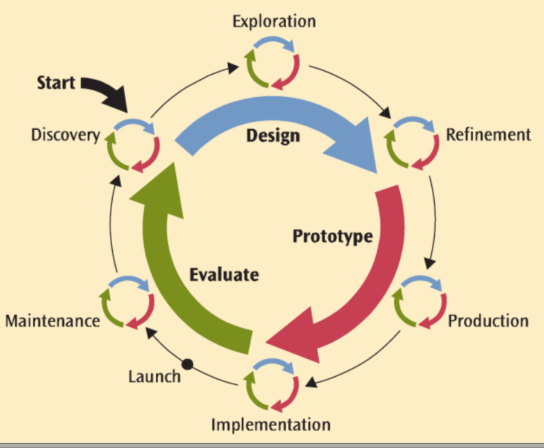
\includegraphics[scale=.35]{Untitled 27.png}}
          \end{figure}
        \begin{itemize}
          \item Fase de descubrimiento: Localizar clientes objetivos y sus necesidades, y los objetivos de negocios.
          \begin{itemize}

      \item Proceso: Determinar el objetivo global. Decidir la proporción de valor del sitio. Hacer lo básico primero.\end{itemize}
  \item Fase de exploración: Generación y evaluación de varios diseños. Reflejan ideas no implementadas.
  \begin{itemize}

      \item Proceso: Generación del mapa del sitio. Evaluar los diseños con los clientes.\end{itemize}
  \item Fase de refinamiento: Una vez seleccionada una idea de diseño, hay que explorarlo. Proporcionar la navegación, las plantillas y el flujo.
  \begin{itemize}

      \item Proceso: Iterativamente refinar, detallar y probar indefinidamente. Determinar tipos de páginas. Determinar aspectos, pero no contenidos.\end{itemize}
  \item Fase de producción: Crear una especificación detalla del sitio. Proporcionar la navegación, las platillas y el flujo.
  \begin{itemize}

      \item Proceso: Definir detalladamente el sitio, creando prototipos interactivos. Evaluación del sitio con clientes.\end{itemize}
        \end{itemize}
      \end{itemize}
  
    
    
\subsubsection{Métodos de inspección} Conjunto de procedimientos que permiten
      evaluar una interfaz a fin de determinar su grado de usabilidad.

\chapter{TEMA 4 - Interacción con las interfaces}

\section{Diseño de la interacción}

    El diseño de la interacción debería tener en cuenta

    \begin{itemize}
    
    \item
      las tareas llevadas a cabo por los usuarios,
    \item
      sus objetivos, y
    \item
      el contexto en el que la interacción ocurre.
    \end{itemize}

    El foco central hacia donde se direcciona el diseño de la
    interacción es comprender cómo los usuarios utilizarán el sistema
    propuesto.

    Para formalizar este proceso, se toman en cuenta varios modelos,
    como los ciclos de vida ya utilizados en Ingeniería del Software.

    
\subsection{Ciclos de vida}
    Pasos cortos con muchas iteraciones.

\subsection{Modelo en Cascada}


    Enfoque linear y secuencial al desarrollo software.

    Hay que primero tener en cuenta los requisitos del sistema y luego
    tener diseño básico antes de empezar la implementación y la fase de
    pruebas.
    \begin{figure}[H]
			\ffigbox[\FBwidth]
			{\caption{Modelo en Cascada}}
			{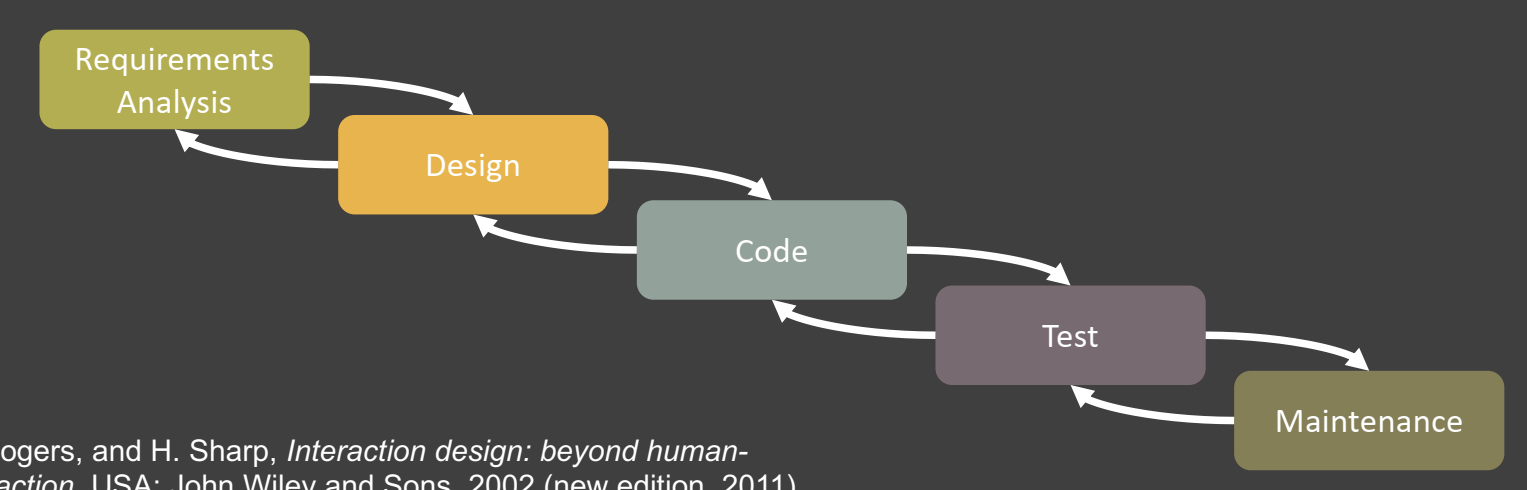
\includegraphics[scale=.25]{Untitled 28.png}}
		\end{figure}

    Los requisitos no se pueden cambiar durante las fases siguientes.

    No es un modelo centrado en el usuario porque no toma en cuenta
    formalmente el usuario.

    
\subsection{Desarrollo ágil}



    Metodología que se centra en hacer que las cosas funcionen más que
    en documentarlas.

    No hay un plan estricto, según se progresa se va cambiando.

    Se centra en el individuo y la interacción antes que la herramienta
    a usar.

    Colaborar con el usuario de forma continua, antes que firmar un
    contrato y

    
\subsection{Diseño ágil}


    Diseñamos e implementamos continuamente, se itera muchas veces.

    FeedBack frecuentes de los clientes que se tienen en cuenta al
    momento para modificar el diseño del sistema.

    El cliente es un miembro del equipo de desarrollo.

    Reunión frecuentes entre los miembros del equipo de diseño.

    Pruebas frecuentes.

    Enfoque: Resolver los problemas o necesidades del cliente.

    
\section{Requisitos: Definición y tipos}

    Necesidades o funcionalidades que hay que cubrir.

    Términos relacionados los requisitos:

    \begin{itemize}
    
    \item
      Recogida de requisitos, tomar del entorno de los requisitos.
    \item
      Pliego de requisitos.
    \item
      Análisis de requisitos, analiza un conjunto inicial, para sacar
      los importantes y ver los duplicados.
    \item
      Ingeniería de requisitos.
    \end{itemize}

    Es una declaración sobre un producto deseado que especifica qué
    debería hacer o cómo debería hacerlo.

    \begin{itemize}
    
    \item
      Ejem: Tiempo de descarga de una página debe ser menor de 5.
    \end{itemize}

    Tienen muchas formas y muchos niveles de abstracción.
\pagebreak

    Tipos de requisitos:

    \begin{itemize}
    
    \item
      Funcionales: Que debe hacer el sistema, relativo al usuario.
    \item
      No funcionales: Restricciones del sistema y su desarrollo,
      relativo a especificación técnica.
    \end{itemize}

    Otra lista más exhaustiva de tipos de requisitos:

    \begin{itemize}
    
    \item
      De datos: tipo, volatilidad, tamaño, persistencia, precisión y
      valor.
    \item
      Del entorno: entorno físico (p. ej. luz y ruido), entorno social
      (p. ej. colaboración), entorno organizacional y entorno técnico
      (p. ej. compatibilidad).
    \item
      Del usuario: talento y habilidades; casual o frecuente; experto o
      novato. (Perfil de usuario).
    \item
      De usabilidad: efectividad, eficiencia, seguridad, utilidad y
      aprendizaje.
    \end{itemize}

\section{Recogida de datos}



    El objetivo es recoger datos suficientes, relevantes y apropiados
    para definir un conjunto estable de requisitos. Entender al usuario
    y el entono para recoger los datos.

    Si ya existe un conjunto de requisito, sirve para expandir,
    clarificar y confirmar ese conjunto.

    Se deben conocer cómo se realizan las tareas en la actualidad, así
    como las metas asociadas, el contexto en el que se realizan y las
    razones de por qué las cosas son como son.

    Técnicas para recoger información:

\subsection{Cuestionarios.}

        QUIS - Questionnaire for User Interface Satisfaction.

        \begin{itemize}
        
        \item
          Evalúa la satisfacción subjetiva con aspectos específicos de
          HCI.
        \item
          Propósitos: Guiar el diseño y rediseño de sistemas; evaluar
          áreas y realizar evaluaciones.
        \end{itemize}
\pagebreak
        CSUQ - Computer System Usability Questionnaire.

        \begin{itemize}
        
        \item
          Mide con 19 preguntas la satisfacción del usuario con respecto
          a la usabilidad.
        \end{itemize}

        PUEU - Perceived Usefulness and Ease of Use.

        \begin{itemize}
        
        \item
          Desarrollo para respaldar el modelo de aceptación de la
          tecnología, utilidad percibida y facilidad de uso.
        \end{itemize}

        NAU - Nielsen's Attributes of Usability

        \begin{itemize}
        
        \item
          ``Learnability'': los sistemas deberían ser fáciles de
          aprender.
        \item
          Eficiencia: los sistemas deberían ser eficientes en su uso.
        \item
          Memorabilidad: los sistemas deberían ser fáciles de recordar.
        \item
          Errores: el sistema debe tener una baja tasa de errores.
        \item
          Satisfacción: el sistema debe ser agradable de usar.
        \end{itemize}

        ASQ - After Scenario Questionnaire

        \begin{itemize}
        
        \item
          Aborda tres componentes importantes de la satisfacción del
          usuario con la usabilidad del sistema: facilidad para
          completar tareas, tiempo para completar una tarea y adecuación
          de la información de soporte.
        \end{itemize}

        PUTQ - Purdue Usability Testing Questionnaire

        \begin{itemize}
        
        \item
          Evalúa 8 factores relevantes en HCI.
        \end{itemize}

        SUMI - Software Usability Measurement Inventory

        \begin{itemize}
        
        \item
          Evalúa la calidad del uso de un producto o prototipo de
          software. Puede ayudar a detectar fallos de usabilidad antes
          de enviar un producto.
        \end{itemize}

        SUS - System Usability Scale

        \begin{itemize}
        
        \item
          Escala Likert de actitud de 10 elementos. Visión global de las
          evaluaciones subjetivas de usabilidad.
        \end{itemize}
\pagebreak
        TAM - Technology Acceptance Model

        \begin{itemize}
        
        \item
          Con un punto de vista totalmente diferente, más orientado a la
          tecnología desarrollada, y uno de los más usados hoy en día.

          \begin{itemize}
          
          \item
            Expectativa de rendimiento
          \item
            Expectativa de esfuerzo
          \item
            Actitud hacia el uso de la tecnología
          \item
            Influencia social
          \item
            Condiciones facilitadoras
          \item
            Autoeficacia
          \item
            Ansiedad
          \item
            Intención de usar el sistema.
          \end{itemize}
        \end{itemize}

        Para diseñar un cuestionario efectivo hay que tener en cuenta el
        texto y la organización de las preguntas.

        \begin{itemize}
        
        \item
          Si las preguntas son difíciles o ambiguas, no obtendrán datos
          útiles.
        \item
          Validez: El cuestionario mide lo que se espera que mida. Han
          sido probado por muchos usuarios.
        \item
          Fiabilidad: Se refiere a la consistencia del cuestionario. Se
          obtendrá una respuesta similar si lo realizase el usuario en
          varios momentos.
        \end{itemize}

        La parte más difícil de diseñar un cuestionario es diseñar el
        piloto

        \begin{itemize}
        
        \item
          La primera versión de un cuestionario casi siempre no va a ser
          la definitiva. Los pilotos son versiones preliminares de los
          cuestionarios
        \item
          Los pilotos se evalúan con una muestra de usuarios y permiten
          a los investigadores diseñar el cuestionario final
          identificando y solucionando posibles problemas.
        \end{itemize}

        Preguntas abiertas:

        \begin{itemize}
        
        \item
          No tienen ningún tipo de opción para las respuestas.
        \item
          Los usuarios tienen que escribir su respuesta. De esta forma
          los usuarios pueden expresar sus puntos de vista y son fáciles
          de preguntar.
        \item
          Son bastante difíciles de analizar debido a la ambigüedad del
          lenguaje natural, y exigen más esfuerzo de los usuarios (por
          ejemplo, para pensar en la respuesta)
        \end{itemize}

        Preguntas cerradas:

        \begin{itemize}
        
        \item
          vienen con unas opciones alternativas de respuestas

          \begin{itemize}
          
          \item
            Check-boxes e intervalos se usan típicamente para respuestas
            como Sí o No o edades (por ejemplo, \textless3 meses, entre
            3 y 6 meses,\textgreater{} 6 meses)
          \item
            Las escalas Likert se usan para medir las opiniones de los
            usuarios (por ejemplo, totalmente de acuerdo, de acuerdo,
            muy en desacuerdo)
          \item
            Las escalas diferenciales semánticas se usan para medir las
            actitudes de los usuarios (por ejemplo, fácil 1- 2-3-4-5
            difícil)
          \item
            Más fáciles de analizar
          \end{itemize}
        \end{itemize}

\subsection{Entrevistas}


        Entrevistar es un intercambio interactivo de hacer preguntas y
        obtener respuestas.

        Las entrevistas solo revelan parte de la información.

        Las entrevistas requieren mucho tiempo y pueden ser caras.

        Las entrevistas requieren preparar el material con mucho cuidado
        para evitar la ambigüedad del lenguaje natural, teniendo en
        cuenta también la variabilidad de las personas y el coste de
        viajar al contexto de los usuarios.

        El control que ejerce el entrevistador sobre la entrevista varía
        según el objetivo de la investigación.

\subsubsection{Entrevistas estructuradas}

        \begin{itemize}
        
        \item
          Se llevan a cabo en una pequeña habitación.
        \item
          Lista predeterminada de preguntas y respuestas (un
          cuestionario) que se lee en voz alta y el usuario tiene que
          responder. El entrevistador juega un papel neutral y toma
          mucho control sobre la entrevista.
        \item
          El trabajo preparatorio es esencial para recoger datos de
          manera específica.
        \item
          Las entrevistas se pueden repetir fácilmente y los resultados
          analizados (estudio estándar).
        \item
          No tienen en cuenta la interacción social entre
          entrevistadores y entrevistados. También pueden ser
          entrevistas telefónicas y en centros comerciales y parques.
        \end{itemize}

\subsubsection{Entrevistas no estructuradas}

        \begin{itemize}
        
        \item
          Conversaciones centradas en un tema.
        \item
          El guion utilizado solo contiene temas principales a abordar
          en la entrevista.
        \item
          Los temas se plantean generalmente a través de preguntas
          abiertas, a diferencia de las entrevistas estructuradas.
        \item
          Otras cuestiones podrían surgir durante la entrevista.
        \item
          Se pueden generar muchos datos contextuales, aun si su
          análisis requiere mucho tiempo por ser conversaciones libres.
        \item
          Hay interacción social entre entrevistado y entrevistador.
        \end{itemize}

\subsubsection{Entrevistas semi-estructuradas}

        \begin{itemize}
        
        \item
          Combinan características de entrevistas estructuradas y no
          estructuradas.
        \item
          El orden de las preguntas no es estricto, a diferencia de las
          entrevistas estructuradas. Otros temas que podrían plantear
          los entrevistados, se pueden añadir a la lista y ser abordados
          en la entrevista.
        \item
          Se pueden incluir también preguntas abiertas, pero estas
          tienden a ser más específicas que las preguntas en entrevistas
          no estructuradas.
        \item
          Los entrevistadores tienen una idea más definida acerca de los
          temas o información que debe recopilarse
        \end{itemize}

\subsubsection{Entrevistas en grupo - Focus group}

        \begin{itemize}
        
        \item
          Consisten en entrevistar a varios usuarios al mismo tiempo en
          un ambiente formal o informal.
        \item
          Tomar el control sobre un grupo de personas es más difícil que
          controlar a una sola persona.
        \item
          El control del entrevistador varía dependiendo del tipo de
          entrevista en grupo. Los focus groups son las entrevistas de
          grupo más usadas.
        \item
          Hay otros tipos de entrevistas en grupo, por ejemplo,
          brainstorming, que requieren menos control que los grupos
          focales.
        \end{itemize}
\subsection{Grupos de interés y talleres}
\subsection{Observación}

        Observación de los usuarios

        \begin{itemize}
        
        \item
          Observar las actividades y participar en ellas
        \item
          Observaciones de primera mano: ``lo que la gente dice que hace
          (es decir, en cuestionarios y entrevistas) y lo que realmente
          hacen tiende a no ser lo mismo''
        \item
          Demasiado tiempo (en antropología, años, en sociología, años y
          meses)
        \item
          Muchos datos
        \item
          Puede ser manifiesta y encubierta
        \end{itemize}

        Revisión de documentos (``Document review''): Revisar los
        documentos de las distintas versiones, para ver si se encuentran
        mejores o alternativas.

        \begin{itemize}
        
        \item
          Reglas y procedimientos.
        \item
          Técnica cuantitativa.
        \item
          Los usuarios no están realmente involucrados.
        \item
          Rutina diaria versus procedimientos.
        \end{itemize}

        Análisis de registros (``Analysis of logs''): Ver registros de
        como el usuario ha usado el sistema.

        \begin{itemize}
        
        \item
          Cómo funciona el sistema (métricas).
        \item
          Técnica cuantitativa.
        \item
          ``Menos'' participación del usuario.
        \item
          Las opiniones no se tienen en cuenta.
        \end{itemize}

\subsection{Estudio de la documentación}
\subsection{Software de Registro}
\pagebreak
    Hay que tener en cuenta que información queremos obtener y cuánto
    tiempo tenemos.
  
    Aspectos a tener en cuanta:

    \begin{itemize}
    
    \item
      La naturaleza de los datos: Cantidad de tiempo y nivel de detalle.
    \item
      La tarea a ser estudiada: Es secuencial o se solapan las
      diferentes subtareas.
    \end{itemize}

    Guías para realizar la recogida de datos:

    \begin{itemize}
    
    \item
      Enfocarla a la identificación de las necesidades de los usuarios.
    \item
      Involucrar a todos los tipos de grupos de usuarios.
    \item
      Involucrar a más de un usuario de esos grupos.
    \item
      Combinación de técnicas.
    \item
      Realizar una prueba piloto de recogida de datos.
    \item
      Compromiso entre la situación idílica y las restricciones de la
      realidad.
    \item
      Recogida de datos práctica.
    \end{itemize}


  \section{Interpretación y análisis de los datos.}

    El objetivo de la interpretación es estructurar y registrar
    descripciones de requisitos.

    Es bueno definir modelos de requisitos que incluyan: identificador,
    tipo, descripción, razón, criterios de adecuación, satisfacción del
    usuario, dependencias, historia, \ldots{}

    Esta información se incluye en documentos o diagramas que tienen
    enlaces al origen de esos requisitos.

    El análisis tiene que ver con la investigación de los distintos
    aspectos del sistema de acuerdo con los requisitos establecidos y
    las técnicas para comprender las metas y los objetivos de los
    usuarios, y comprender en profundidad los requisitos.

    \begin{itemize}
    
    \item
      Funcionales, de datos, diagramas de clases y de secuencia,
      \ldots{}
    \item
      Descripción de tareas: Describen las tareas por las que el sistema
      va a ser aceptado.
    \item
      Análisis de tareas: La información recogida establece la base de
      las prácticas de análisis para evaluar las tareas definidas, como
      en HTA y GOMS.
    \end{itemize}

\subsection{Descripción de tareas}

\subsubsection{Escenarios}

      Descripción informal de actividades o tareas humanas que permiten
      la exploración y discusión de contextos, necesidades y requisitos.

      Los primeros escenarios los construyen los usuarios habitualmente.

      Se basa en una narración en la que aparecen: Actores, Actividades
      y Objetos.
 
\subsubsection{Tipo de representaciones para escenarios}


      Narrativa: Una historia completa de la interacción con el sistema
      existente.

      Diagrama de flujo: Una representación gráfica de las series de
      acciones y decisiones.

      Textos de los procedimientos: Una descripción paso a paso de las
      acciones del usuario y las respuestas del sistema.

      Storyboard: Una narración gráfica de una historia en cuadros
      consecutivos. Suele usar para la realización de escenarios de
      interacción.

\subsubsection{Casos de uso}

      Enfatiza la tarea del usuario más que la interacción con el
      sistema.

      Se enfoca en la interacción entre el usuario y el sistema, desde
      la perspectiva del usuario.

      Existen un escenario en los casos de uso que indican el camino a
      través de un conjunto concreto de condiciones.

      Un caso de uso se asocia a un actor, y pretende describir el
      objetivo del actor que usa el sistema.

      El caso de uso principal se llama rumbo normal.

      Otras alternativas se llaman rumbos alternativos.
\pagebreak
\subsection{Análisis de tareas}


    Técnicas para analizar tareas:

    
\subsubsection{Análisis Jerárquico de Tareas - HTA}
      
      Dividir una tarea en
      subtareas de forma recursiva. Romper las tareas grandes en tareas
      más pequeñas.

      
        Se focaliza en las acciones observables y físicas.

        Se basa en la división de tareas en subtareas.

        Proceso:

        \begin{itemize}
        
        \item
          Comenzar con un objetivo de usuario del que identificar las
          tareas principales que hay que realizar para lograrlo.

          \begin{itemize}
          
          \item
            El objetivo es el punto 0. que sobresale un poco de resto.
          \end{itemize}
        \item
          Las tareas se subdividen en subtareas, hasta llegar al grado
          de granularidad requerido, las tareas que hace el usuario.

          \begin{itemize}
          
          \item
            Se ponen como sub puntos dentro las tareas, 1.1.
          \end{itemize}
        \item
          Las subtareas se agrupan en un plan. Cada plan especifica como
          se pueden realizar las tareas en una situación real.

          \begin{itemize}
          
          \item
            Cada plan solo tiene tareas de que están dentro de su punto.
          \item
            Siempre hay Plan 0. que puede usar todas las tareas, pero no
            subtareas.
          \item
            Si hay subtareas, el plan es el número de las tareas y solo
            contiene sus subtareas.
          \item
            Ejem: Plan 2: hacer 2.1-2.4-2.5. Si no se identifica el
            libro hacer 2.2-2.3-2.4-2.5
          \end{itemize}
        \end{itemize}

        Un HTA está completo si está en texto y gráfico.
        \begin{figure}[H]
          \ffigbox[\FBwidth]
          {\caption{HTA}}
          {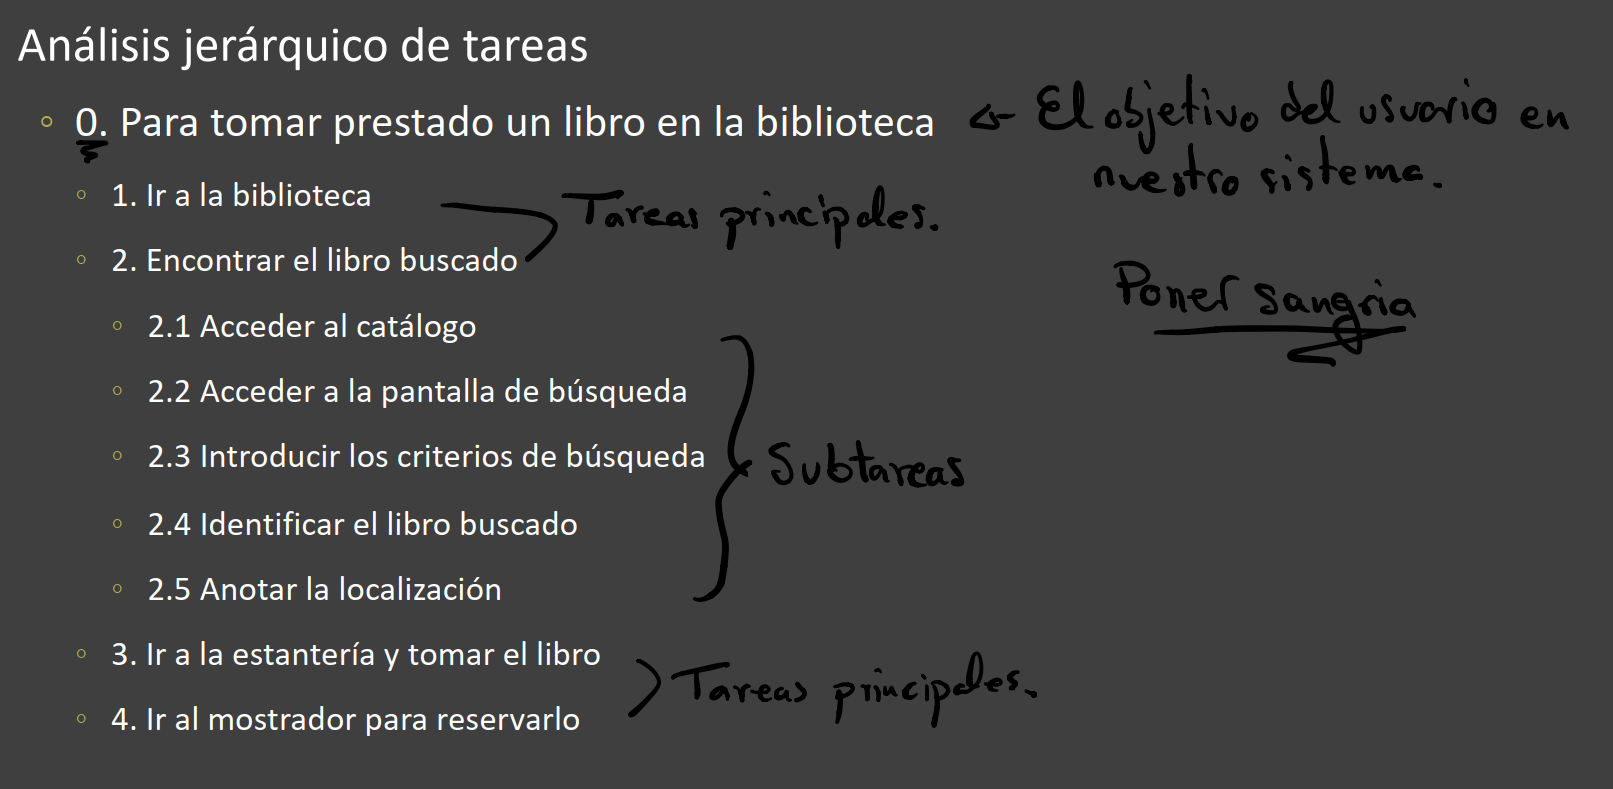
\includegraphics[scale=.25]{Untitled 29.png}}
        \end{figure}
        \begin{figure}[H]
          \ffigbox[\FBwidth]
          {\caption{Diagrama HTA}}
          {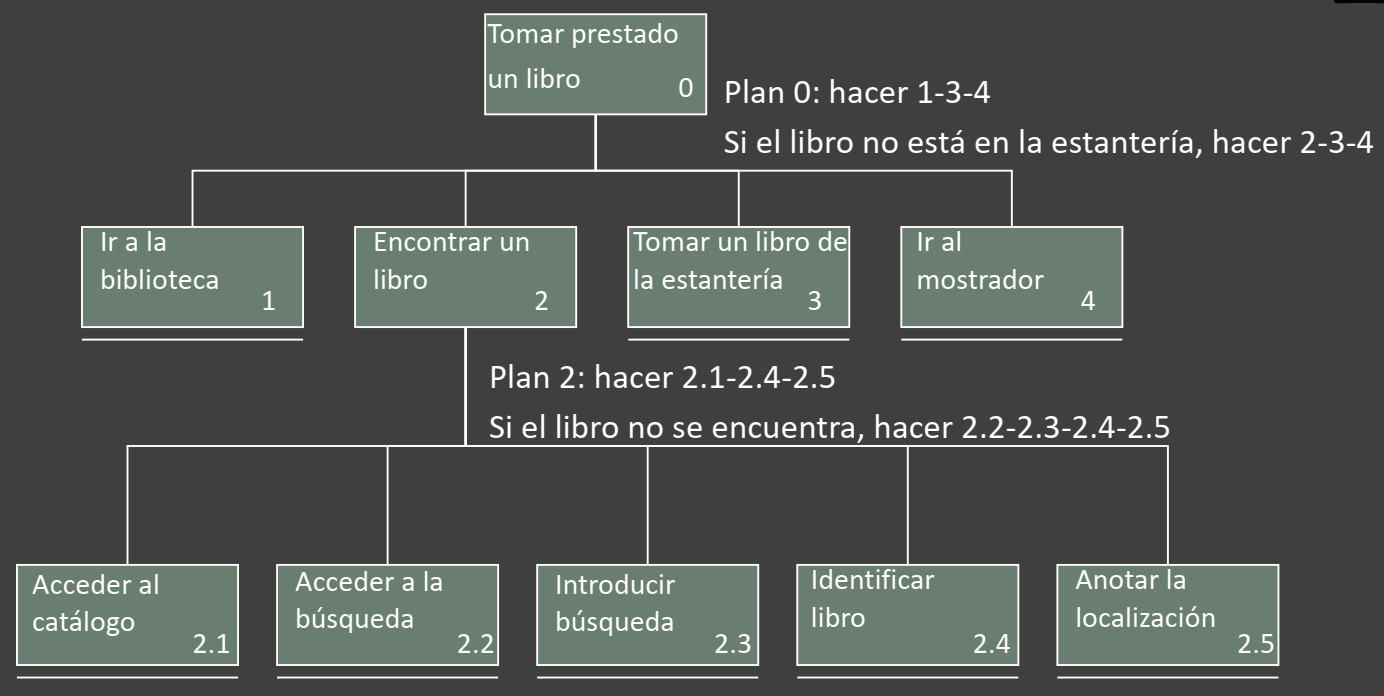
\includegraphics[scale=.3]{Untitled 30.png}}
        \end{figure}
        Se ponen las tareas como hijas de las tareas padre, y cuando no
        tienen subtareas se pone una línea horizontal debajo.

        Se ponen los planes próximos a la tarea a la que corresponde.

        \pagebreak
\subsubsection{Modelos predictivos}
      Modelos a priori para definir una
      aproximación de las acciones que los usuarios ejecutaran antes de
      involucrar los usuarios mismos en test reales.

\paragraph{Model Human Processor - MHP}
         Se usa para hacer predicciones
        sobre como el usuario ejecuta las tareas.

        
          Se compone de un conjunto de memoria y procesadores que
          funcionan siguiendo a unos principios de operación.

          Sistema de percepción:

          \begin{itemize}
          
          \item
            Sensores: ojos, oídos.
          \item
            Buffer: Visual memory store, Auditory memory store.
          \item
            Sistema cognitivo: Working memory o short-term memory,
            Long-term memory.
          \item
            Sistema motor: sistema brazo-mano-dedo, sistema cabeza-ojo.
          \end{itemize}

          
\paragraph{Goals, Operators, Methods and Selection rules - GOMS} 
Tiene objetivo el modelo del conocimiento y de los procesos cognitivos
        que se producen cuando el usuario interactúa.

        \begin{itemize}
        \item
          Goals: Estados concretos que el usuario quiere conseguir.
        \item
          Operators: Procesos cognitivos y acciones físicas para lograr
          esas metas.
        \item
          Methods: Procedimientos aprendidos para conseguir una meta.
        \item
          Selection rules: Determinan que método elegir cuando hay más
          de un escenario en una tarea.
        \end{itemize}

          Se utiliza mucho para comparar sistemas distintos.

          Funciona bien para análisis sencillos, pero no para complejos.

          Se necesita una herramienta que automatice el proceso.
        \begin{figure}[H]
          \ffigbox[\FBwidth]
          {\caption{Ej. GOMS}}
          {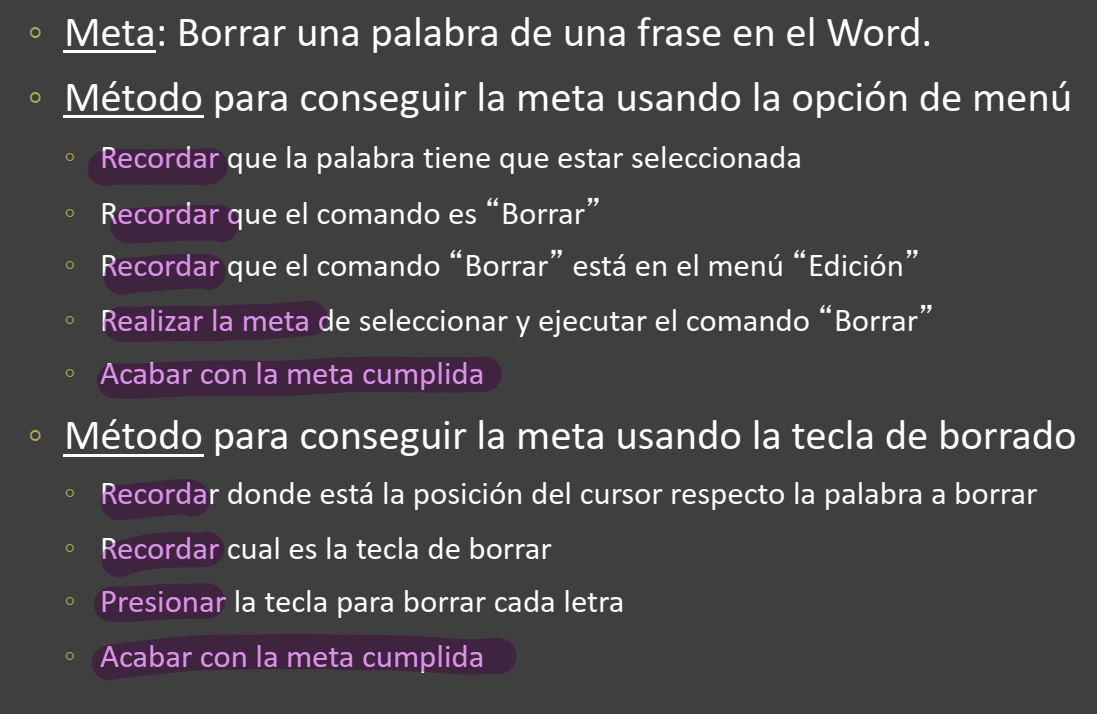
\includegraphics[scale=.3]{Untitled 31.png}}
        \end{figure}
        \begin{figure}[H]
          \ffigbox[\FBwidth]
          {\caption{Ej. GOMS}}
          {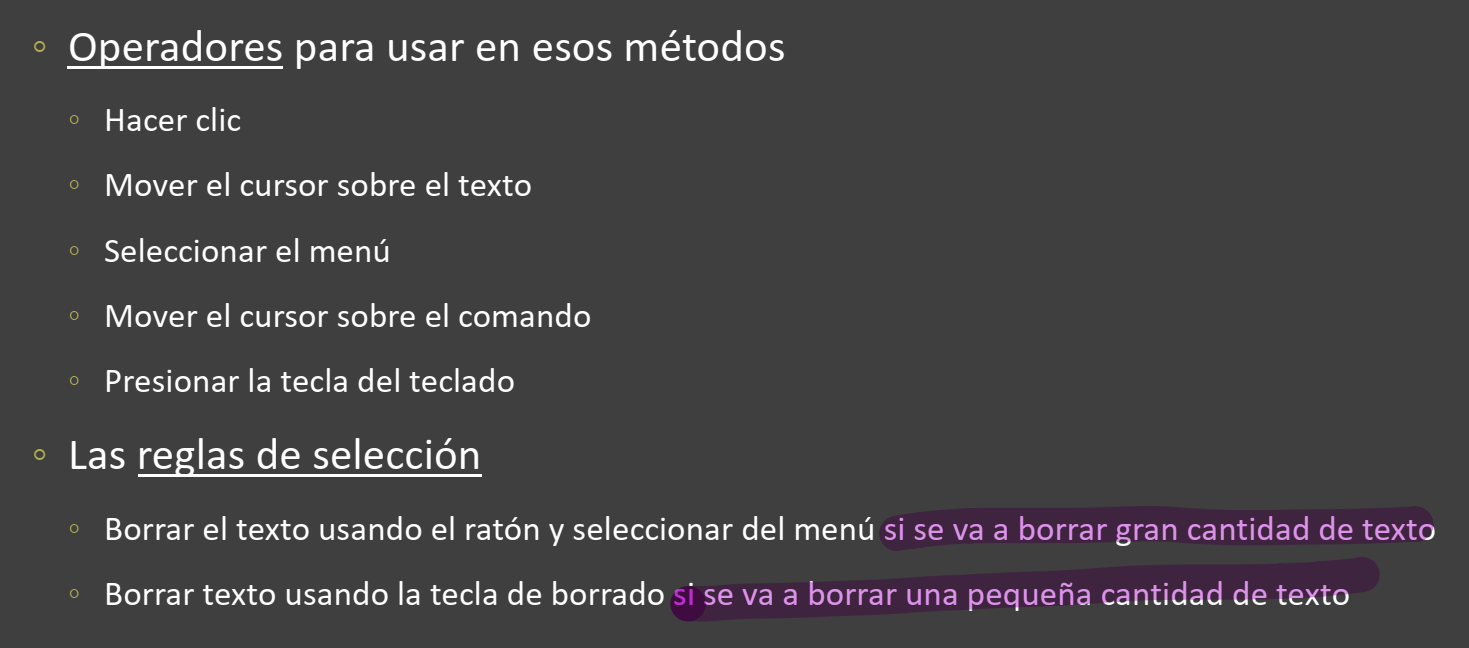
\includegraphics[scale=.25]{Untitled 32.png}}
        \end{figure}
        \pagebreak
\paragraph{Keystroke-Level Model KLM - KLM} 
Evalúa el rendimiento de un sistema.


          Asigna un tiempo determinado a cada acción, salvo para el
          ratón que depende de la distancia entre el punto de partida y
          de llegada.

          Para un sistema típico, hay 7 componentes:

          \begin{itemize}
          
          \item
            K (0.2 s) -- press a key or mouse button. Presionar una
            tecla.
          \item
            P (1.1 s) -- point with mouse. Apuntar con el ratón.
          \item
            H (0.4 s) -- home on keyboard, mouse or other device. Mover
            la mano al dispositivo.
          \item
            M (1.35 s) - mentally prepare. Tiempo de preparación mental
            para hacer la acción.
          \item
            R (t) - system response time. Respuesta del sistema.
          \item
            B (0.1 s) - press or release mouse button. Pulsar o soltar
            botón del ratón.
          \item
            BB (0.2 s) - click mouse button. Hacer clic.
          \end{itemize}

          Reglas:

          \begin{itemize}
          
          \item
            M al comenzar la tarea o cuando se cambia de tarea.
          \item
            H cada vez que se cambia de dispositivo.
          \end{itemize}

\paragraph{Ley de Fitt}
        El tiempo requerido para conseguir un objetivo es
        proporcional a la distancia y al tamaño del objetivo (tamaño
        físico, una barra, botón\ldots)


        
          Las opciones más importantes deben tener mayor tamaño o ser
          más visibles que las secundarias.

          La localización también es importante.

          ID - Índice de dificultad: Se define como la dificultad de una
          tarea en términos de distancia y anchura.
          \(ID = log_2 ( \frac {D} {W} + 1)\)

          \begin{itemize}
          
          \item
            D: Distancia hasta el centro del objetivo.
          \item
            W: Ancho del objetivo medido sobre el eje del movimiento.
          \end{itemize}

          MT - Tiempo medio: Necesario para alcanzar un elemento de la
          interfaz. \(MT = a+b*ID\)

          \begin{itemize}
          
          \item
            a: tiempo de inicio o parada en segundos.
          \item
            b: velocidad inherente del dispositivo.
          \end{itemize}

          
\paragraph{Ley de Hick}
El tiempo que se tarda en tomar una decisión
        aumenta a medida que se incrementa el número de alternativas.

          El tiempo para elegir una opción entre n alternativas.
          \(T=a+b*log_2 (n+1)\)

          \begin{itemize}
          
          \item
            a y b coeficiente que se determina experimentalmente.
          \end{itemize}

          Teniendo todas las opciones en el menú la misma probabilidad
          de ser elegidos.

          En web:

          \begin{itemize}
          
          \item
            Se utilizan colores saturados para llamar la atención sobre
            algo.
          \item
            Utiliza tipografía y tamaños neutros y equilibrados si
            deseas dar a elegir entre varias opciones del mismo nivel.
          \item
            Utiliza el movimiento y la interacción para destacar
            poderosamente.
          \item
            Utiliza el equilibrio de espacios, no situar elementos de
            igual importancia en lugares muy distantes.
          \item
            Utiliza buena semántica a la hora de seleccionar las
            palabras que representan las opciones.
          \end{itemize}

          
        

\section{Diseño conceptual}

    Tiene como objetivo transformar los requisitos y necesidades del
    usuario en un modelo conceptual.

    Un modelo conceptual es una descripción del sistema propuesto como
    un conjunto integrado de ideas y conceptos sobre qué debería hacer,
    cómo debería comportarse y cómo debe ser su apariencia.
\vspace{-0.5cm}
    \begin{itemize}
    
    \item
      Los usuarios realizan su modelo mental.
    \item
      Los diseñadores realizan un diseño conceptual.
    \end{itemize}

    Etapa muy ligada a la recogida de información, hay que diferenciar
    entre que debería hacer y solución adoptada.

    Guías a tener en cuenta:
    \vspace{-0.5cm}

    \begin{itemize}
    
    \item
      Mantener una mente abierta sin olvidar a los usuarios y su
      contexto.
    \item
      Discutir las ideas como los usuarios del sistema.
    \item
      Usar prototipos de baja calidad para conseguir información
      rápidamente.
    \item
      Iterar, iterar e iterar.
    \end{itemize}

    Manera de pensar el modelo conceptual:

    \begin{itemize}
    
    \item
      Modo de interacción: Forma en que el usuario invoca acciones
      cuando interactúa con el dispositivo.

      \begin{itemize}
      
      \item
        Depende de la actividad que el usuario va a llevar a cabo con
        el producto.
      \item
        Modo de interacción vs. Estilo de interacción:

        \begin{itemize}
        
        \item
          Estilo de interacción: Tipo de IU y la interacción que
          implica.
        \item
          Modo de interacción: Como interactúa con el producto, como
          tipo de acción.
        \end{itemize}
      \item
        Tipos:

        \begin{itemize}
        
        \item
          Basado en actividades:

          \begin{itemize}
          
          \item
            Instrucciones: Dar instrucciones y el sistema responde.
          \item
            Conversación: Un diálogo entre el usuario y el sistema, el
            usuario consulta y el sistema le responde dando opciones o
            lugar a continuar.
          \item
            Manipulación y navegación: Manipular, moverse por los
            elementos.
          \item
            Exploración y hojeado: Moverse por las opciones o el
            contenido.
          \end{itemize}
        \item
          Basado en objetos:

          \begin{itemize}
          
          \item
            Analogías: Por asociación de los elementos del sistema con
            el mundo real. Como un carrito de la compra o escritorio.
          \end{itemize}
        \item
          Otras alternativas:

          \begin{itemize}
          
          \item
            Modelos orientados a los procesos: No se puede identificar
            un trabajo fundamental. No realiza una tarea concreta.
          \item
            Modelos orientados a productos: Productos son identificables
            individualmente. No se parte de 0, se tiene un producto y se
            trabaja sobre él, se trabaja para mejorarlo o añadir cosas.
          \end{itemize}
        \end{itemize}
      \end{itemize}
    \item
      Existencia de una metáfora:

      \begin{itemize}
      
      \item
        Tienen como objetivo combinar conocimiento familiar con otro
        nuevo, de manera que ayudan al usuario a comprender el sistema y
        balancear la combinación de elementos nuevo con elementos
        conocidos.
      \item
        Proceso para seleccionar una buena metáfora:

        \begin{itemize}
        
        \item
          Comprender qué hará el sistema.
        \item
          Identificar que parte del sistema pueden causar problemas.
        \item
          Generar metáforas.
        \end{itemize}
        \pagebreak
      \item
        Cuestiones a responder por una posible metáfora:

        \begin{itemize}
        
        \item
          Estructura.
        \item
          Relevancia.
        \item
          Representación.
        \item
          Comprensión, fácil de entender por todos.
        \item
          Extensibilidad, si se puede usar en más lugares.
        \end{itemize}
      \end{itemize}
    \item
      Paradigma de interacción a utilizar:

      \begin{itemize}
      
      \item
        Filosofías de diseño que ayudan a desarrollar el producto.
      \item
        Dejar todo de lado y pensar cómo se haría la interacción de la
        forma más fácil y cumpliendo los objetivos del usuario.
      \end{itemize}
    \end{itemize}

    Sirven para tener una visión del producto. Pensar de una manera
    ideal como lograr el objetivo y más adelante se pondrán las
    restricciones.

    Estas ideas deben ser pensadas antes de realizar un prototipo o de
    ser evaluadas con los usuarios.

    Aspectos a tener en cuenta.

    \begin{itemize}
    
    \item
      Tecnologías a utilizar.
    \item
      Interfaces a usar.
    \item
      Qué conceptos tienen que ser comunicados y cómo se estructuran,
      relacionan y presentan.
    \end{itemize}

\chapter{TEMA 5 - Paradigma de interacción}

\includepdf[pages=-]{docs/tema5.pdf}

\part{Práctica}
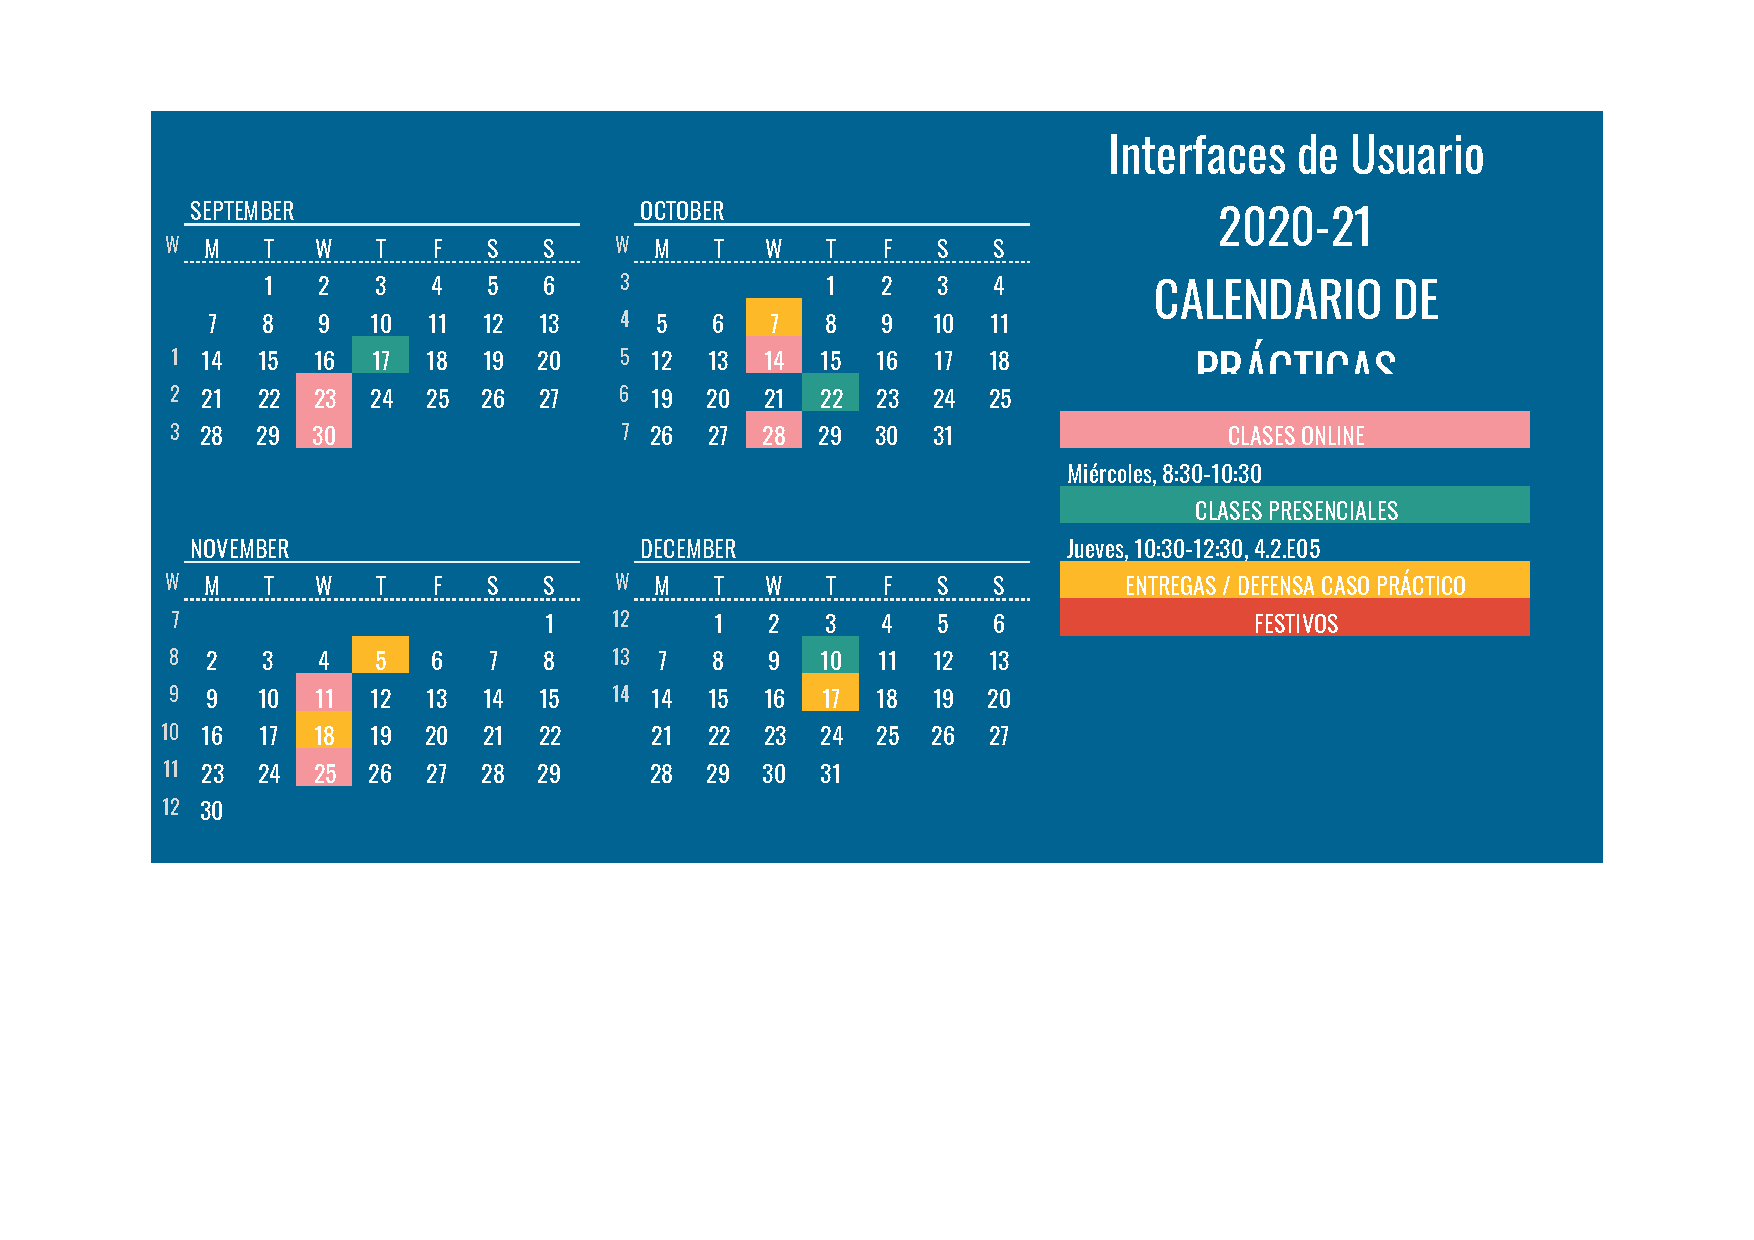
\includepdf[pages=-]{docs/81-IU-cronograma_-_2020.pdf}

\chapter{Tema 1}

  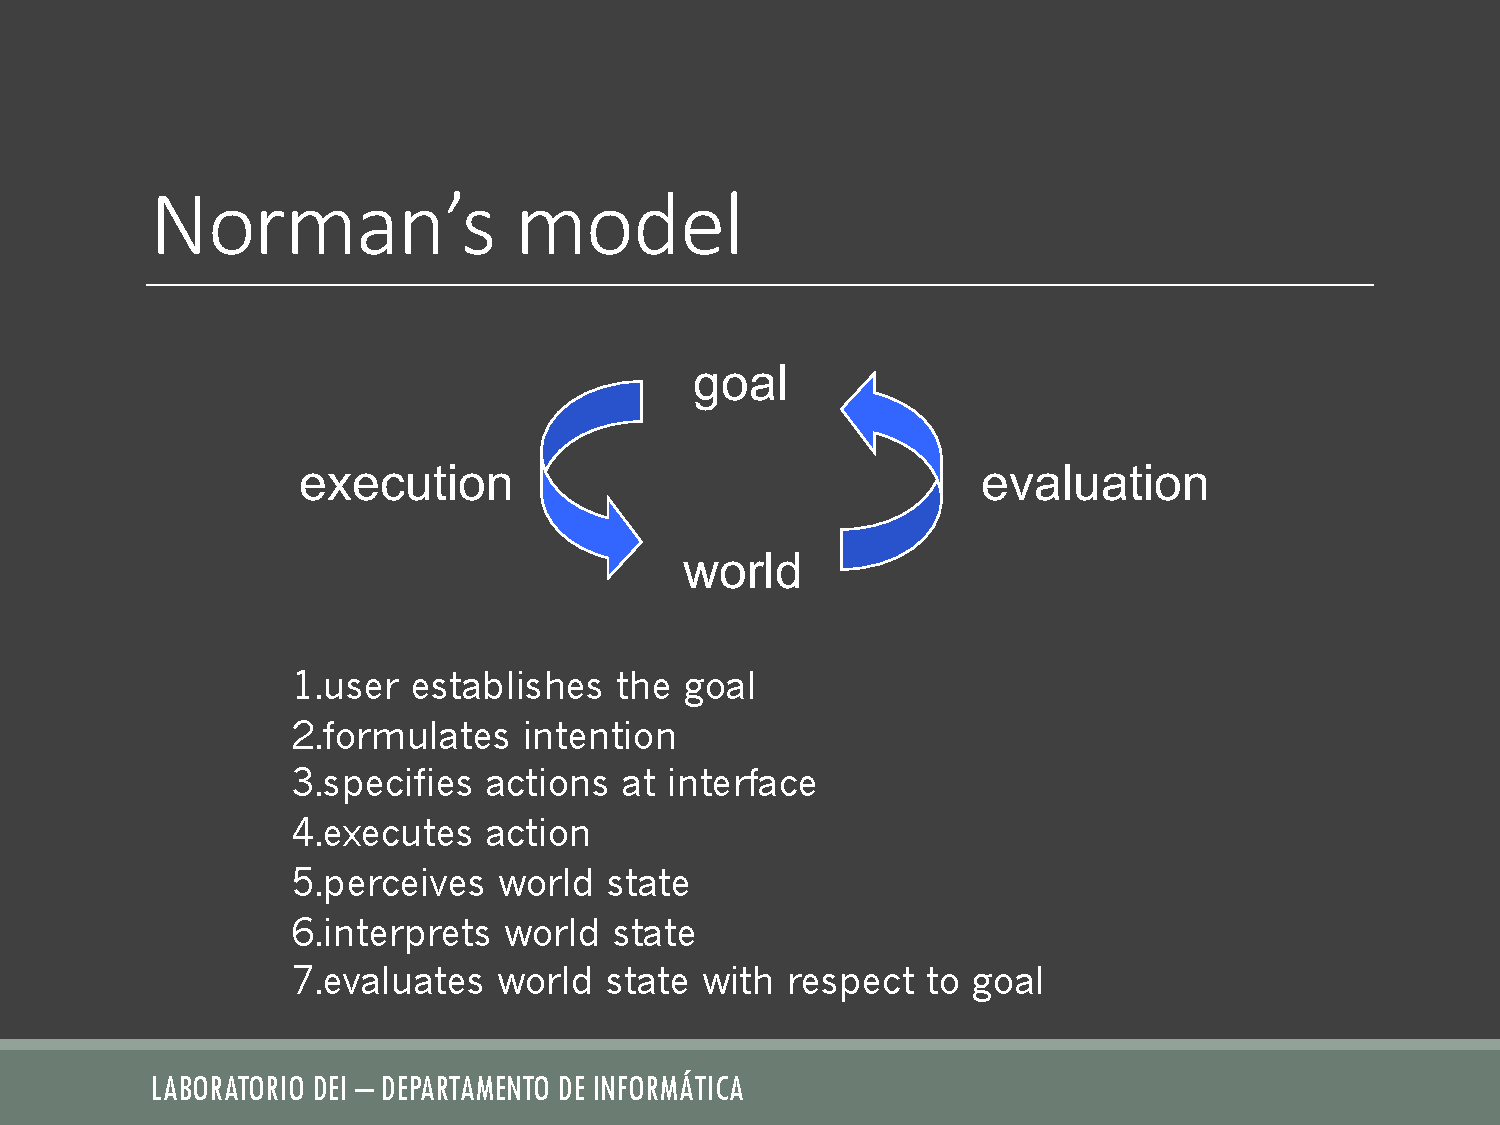
\includepdf[pages=-]{docs/ejemplo-modelo-Norman.pdf}

  \includepdf[pages=-]{docs/Ejercicio1-ModeloNorman.pdf}

\chapter{TECNOLOGÍAS WEB - HTML5 Y CSS3}

  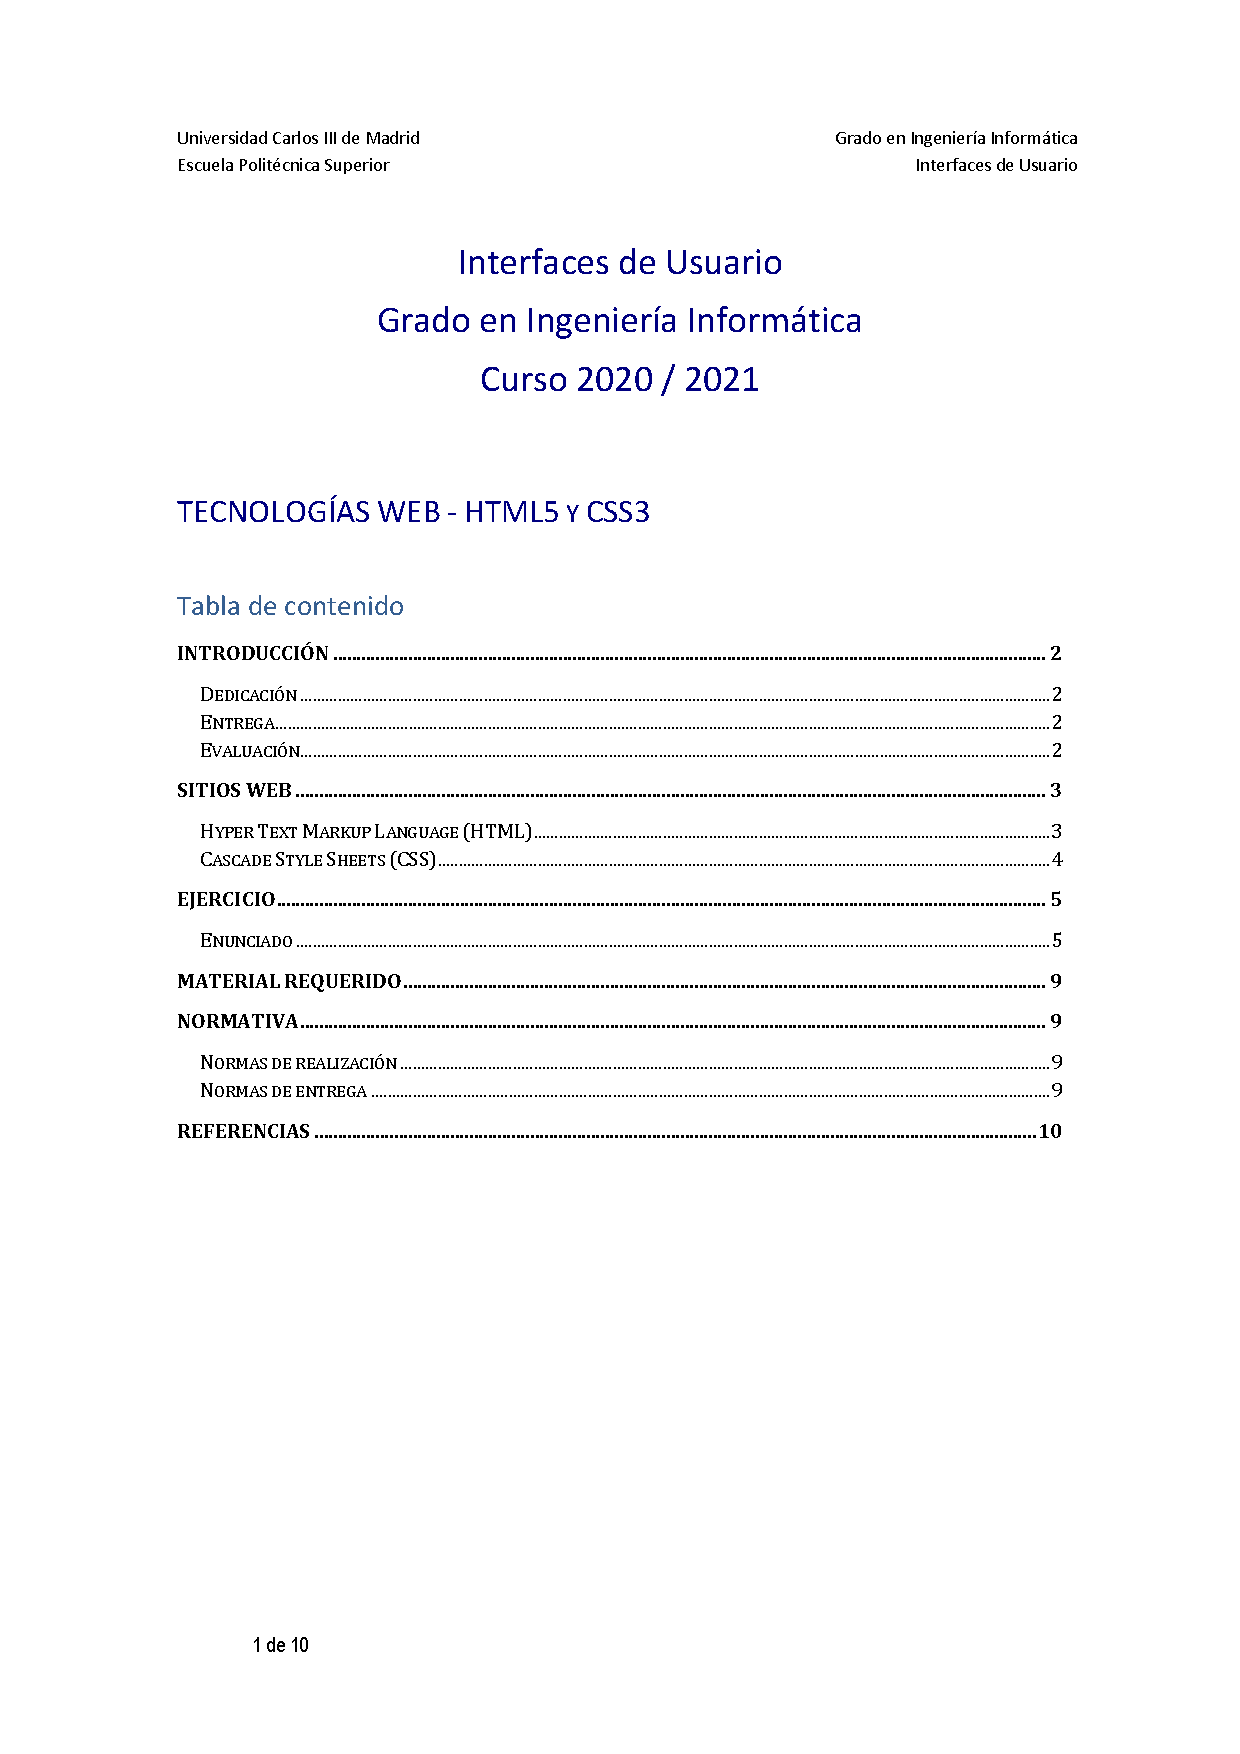
\includepdf[pages=-]{docs/ep01-enunciado.pdf}

  \begin{itemize}
  
  \item
    La web surge nace sobre el año 94 con Tim Berners-Lee en CERN para
    poder conectar todos los ordenadores para compartir datos sin la
    necesidad de un dispositivo físico. A partir de ahí la idea fue
    comprada por empresas y universidades.
  \item
    Diferencia entre web e internet

    \begin{itemize}
    
    \item
      WEB: Es una colección de páginas web con hipervínculos que
      establecen conexiones entre ellas.
    \item
      Internet: Red de ordenadores.
    \end{itemize}
  \item
    WWW: World Wide Web= Red Informática Global.
  \end{itemize}

\section{Arquitectura cliente-servidor}

  El cliente pide información al servido, este se la entrega y la
  muestra al cliente. Se realiza mediante el protocolo HTTP.

  \begin{itemize}
  
  \item
    Protocolo HTTP: En la arquitectura cliente servidor, el cliente
    envía datos al servidor a través del protocolo HTTP. El servidor
    responde con la información solicitada codificada en HTML. El
    cliente interpreta el código HTML, ya que hay por ejemplo diferente
    horas según el país.
  \item
    El cliente se conecta mediante una URL - Uniform Resource Locator,
    secuencia de caracteres que sigue un formato estándar y que se usa
    para localizar recursos en los servidores.
  \end{itemize}

\section{HTML - Hypertext Markup Language}

  Es un lenguaje de marcado estándar para codificar páginas web.

  \begin{itemize}
  
  \item
    Se centra en definir la estructura de una página web.
  \item
    Se compone de una serie de elementos llamados etiquetas que indican
    al navegador la función de la información contenida.
  \end{itemize}
\pagebreak
\begin{lstlisting}[language=HTML]
<!DOCTYPE html>
<html>
  <head>
    <title>Page Title</title>
  </head>
  <body>
    <h1>First Heading</h1>
    <h1 style="color:blue">First Heading in blue</h1>
    <p>This is a paragraph</p>
    <p><a href="https://www.w3schools.com/">Acceder a w3school</a></p>
    <img src="fotoEnLocal.png" alt="InfoFoto" width="500" heigh="333"/>
  </body>
</html>
\end{lstlisting}

\section{CSS}

  Nos permite realizar plantillas de estilo, para poder modificar y
  realizar cambios más grandes a la web completa.

  Clase: class=``nombre'' .nombre\{\} Definir partes del código que
  varíen de las generales.

  Identificador: id=``nombre'' \#nombre\{\} Se puede usar una sola vez.

  Padre \textgreater{} hijo: Se aplican reglas de estilo, para lo tipo
  hijo que están dentro del tipo padre.

  Partes:

  Content: El texto

  Padding: Margen interior.

  Border: Límite entre margen interior y exterior.

  Margin: Margen exterior.

  div: Cajas sin formato.

  clear:both; Limpiar los float para que no se meta en el espacio en
  blanco.

\section{Consortium W3C}

    Es la organización internacional para la creación de estándares web.
    Por ejemplo, poner la etiquetas de cerrado siempre.

    Fue fundada por Tim Berners-Lee en 1994

    Desarrolla estándares de lenguaje como HTML y CSS.

\chapter{JavaScript}

  En un archivo .js

  Mejor usar .addEventListener(evento, acción) que poner en el HTML
  atributos.

  Crear funciones que se llamen, no se que se ejecuten nada más se
  cargue.

\chapter{Prototipado}
\includepdf[pages=-]{docs/Ejercicio2-Prototipado-100405951.pdf}

\includepdf[pages=-]{docs/Ejercicio3-HeuristicasPatrones-100405951.pdf}

\includepdf[pages=-]{docs/Ejercicio4-HTAGOMS-100405951.pdf}

\end{document}